\providecommand{\qcOne}{\mathbf{1}}   %
\providecommand{\qcor}[1]{\ulcorner#1\urcorner}   %

\section{可表示逗号∞-范畴}\label{sec:representable-comma-infinity-categories}

定义 3.4.1 为任何\trCospan{}构造了一个\trCommaInfinityCategory{}。%
在\trCospan{}的一条腿为恒同的特殊情形，这提供了两种对偶机制，把∞-范畴之间的一个%
\trFunctor{}编码为一个∞-范畴本身。

\begin{definition}[左表示与右表示]\label{def:left-right-representations}
任何\trFunctor{} $f\colon A\to B$ 都作为一个\trCommaInfinityCategory{}具有一个\textbf{左表示}%
（left representation）与一个\textbf{右表示}（right representation），如下左与下右所示：
\begin{center}
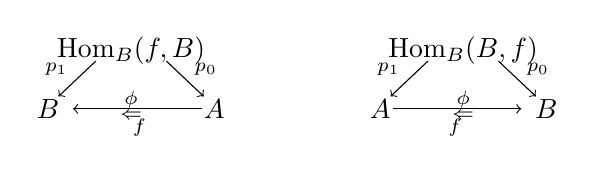
\begin{tikzpicture}[x=1.5em,y=1.5em]
  \node (hom) at (0,2.2) {$\mathrm{Hom}_B(f,B)$};
  \node (b) at (-2.0,0.8) {$B$};
  \node (a) at (2.0,0.8) {$A$};
  \draw[->] (-0.85,1.95) -- (-1.75,1.1);
  \node at (-1.8,1.75) {$\scriptstyle p_{1}$};
  \draw[->] (0.85,1.95) -- (1.75,1.1);
  \node at (1.8,1.75) {$\scriptstyle p_{0}$};
  \node at (0,1.02) {$\scriptstyle\phi$};
  \node at (0,0.64) {$\scriptstyle\Leftarrow$};
  \draw[->] (1.7,0.8) -- (-1.4,0.8);
  \node at (0.2,0.34) {$\scriptstyle f$};
  \node at (4.0,1.5) {\qquad};
  \begin{scope}[shift={(8.0,0)}]
  \node (hom) at (0,2.2) {$\mathrm{Hom}_B(B,f)$};
  \node (a) at (-2.0,0.8) {$A$};
  \node (b) at (2.0,0.8) {$B$};
  \draw[->] (-0.85,1.95) -- (-1.75,1.1);
  \node at (-1.8,1.75) {$\scriptstyle p_{1}$};
  \draw[->] (0.85,1.95) -- (1.75,1.1);
  \node at (1.8,1.75) {$\scriptstyle p_{0}$};
  \node at (0,1.02) {$\scriptstyle\phi$};
  \node at (0,0.64) {$\scriptstyle\Leftarrow$};
  \draw[->] (-1.7,0.8) -- (1.4,0.8);
  \node at (-0.2,0.34) {$\scriptstyle f$};
  \end{scope}
\end{tikzpicture}
\end{center}
\end{definition}

其中，为节省版面，我们把上左所示的 $f$ 的\textbf{左\trCommaCone{}}（left comma cone）%
与上右所示的 $f$ 的\textbf{右\trCommaCone{}}（right comma cone）画作居于三角形而非%
方形之中。

由命题 3.4.11，\trCommaCone{}的弱\trUniversalProperty{}把\textbf{逗号\trSpan}（comma span）%
在余定义域对象之积上直至\trFiberedEquivalence{}刻划。于是：

\begin{definition}\label{def:left-right-representable}
给定一个\trCospan{} $C\xrightarrow{\;g\;}A\xleftarrow{\;f\;}B$，若存在\trFunctor{}%
$\ell\colon B\to C$ 使得
\[
\mathrm{Hom}_A(f,g)\simeq_{C\times B}\mathrm{Hom}_C(\ell,C)
\]
则称\trCommaInfinityCategory{} $\mathrm{Hom}_A(f,g)\twoheadrightarrow C\times B$ 是\textbf{左可表示的}%
（left representable）；若存在\trFunctor{} $r\colon C\to B$ 使得
\[
\mathrm{Hom}_A(f,g)\simeq_{C\times B}\mathrm{Hom}_B(B,r)
\]
则称它是\textbf{右可表示的}（right representable）。%
\end{definition}

在本节中，我们证明一个可表示性定理：\trCommaInfinityCategory{} $\mathrm{Hom}_A(f,g)$ 是右可表示的，%
当且仅当 $g\colon C\to A$ 沿 $f\colon B\to A$ 具有一个\textbf{绝对右提升}%
（absolute right lifting），此时表示\trFunctor{} $r\colon C\to B$ 即定义出所断言的\trLifting{}。%
我们用三则定理来证明这一结果，每一则都强化前一则的陈述。

第一则定理刻划了那些定义绝对右提升图表的\trNaturalTransformation{}——如下所示
\begin{center}
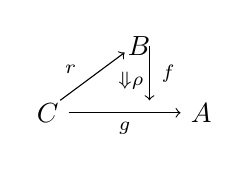
\begin{tikzpicture}[x=1.5em,y=1.5em]
  \node (b) at (2.2,1.6) {$B$};
  \node (c) at (0,0) {$C$};
  \node (a) at (3.7,0) {$A$};
  \draw[->] (0.3,0.3) -- (1.85,1.45);
  \node at (0.55,1.05) {$\scriptstyle r$};
  \node at (2.0,0.78) {$\scriptstyle\Downarrow\rho$};
  \draw[->] (2.45,1.6) -- (2.45,0.3);
  \node at (2.9,0.95) {$\scriptstyle f$};
  \draw[->] (0.5,0) -- (3.2,0);
  \node at (1.85,-0.36) {$\scriptstyle g$};
\end{tikzpicture}
\end{center}
\begingroup
\emergencystretch=3em
——把它们刻划为在\trCommaInfinityCategory{}之间诱导出\trFiberedEquivalence{} $\mathrm{Hom}_B(B,r)\simeq_{C\times B}\allowbreak\mathrm{Hom}_A(f,g)$ 的那些\trNaturalTransformation{}。%
第二则定理证明：\trFunctor{} $r$ 定义 $g$ 穿过 $f$ %
的一个绝对右提升，恰好当 $\mathrm{Hom}_A(f,g)$ 由 $r$ 右表示时；其差别在于无须提供任何%
\trNaturalTransformation{} $\rho\colon fr\Rightarrow g$。最后一则定理给出一个一般的右可表示性判别法，%
可用于在不先验指定表示\trFunctor{} $r$ 的情形下构造 $\mathrm{Hom}_A(f,g)$ 的右表示。%
对偶的结果刻划了左可表示的\trCommaInfinityCategory{}。
\par\endgroup

\begin{theorem}\label{thm:absrl-equivalence}
下左三角定义一个绝对右提升图表，当且仅当其诱导出的下右\trFunctor{}%
\begin{rveq}\label{eq:absrl-induced-map}
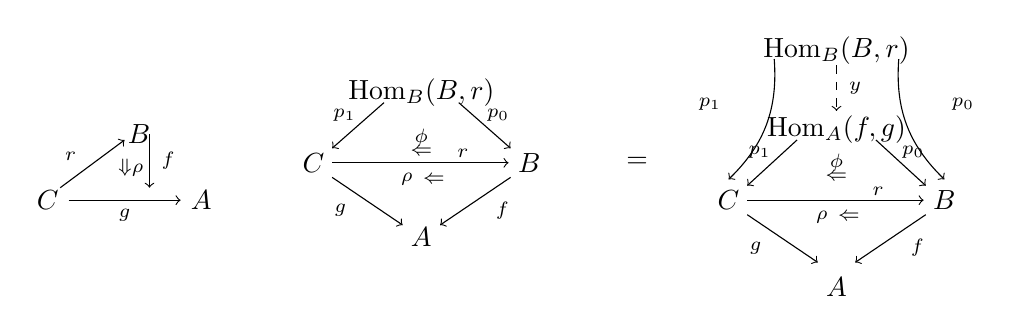
\begin{tikzpicture}[x=1.5em,y=1.5em,baseline=(current bounding box.center)]
  \node (b1) at (0.6,1.6) {$B$};
  \node (c1) at (-1.6,0) {$C$};
  \node (a1) at (2.1,0) {$A$};
  \draw[->] (-1.3,0.3) -- (0.25,1.45);
  \node at (-1.05,1.05) {$\scriptstyle r$};
  \node at (0.4,0.78) {$\scriptstyle\Downarrow\rho$};
  \draw[->] (0.85,1.6) -- (0.85,0.3);
  \node at (1.3,0.95) {$\scriptstyle f$};
  \draw[->] (-1.1,0) -- (1.6,0);
  \node at (0.25,-0.36) {$\scriptstyle g$};
  \node at (3.4,0.8) {$\rightsquigarrow$};
  \begin{scope}[shift={(7.4,0.9)}]
  \node (hom) at (0,1.7) {$\mathrm{Hom}_B(B,r)$};
  \node (c) at (-2.6,0) {$C$};
  \node (b) at (2.6,0) {$B$};
  \node (a) at (0,-1.8) {$A$};
  \draw[->] (-0.9,1.45) -- (-2.15,0.35);
  \node at (-1.85,1.15) {$\scriptstyle p_{1}$};
  \draw[->] (0.9,1.45) -- (2.15,0.35);
  \node at (1.85,1.15) {$\scriptstyle p_{0}$};
  \node at (0,0.6) {$\scriptstyle\phi$};
  \node at (0,0.26) {$\scriptstyle\Leftarrow$};
  \draw[->] (-2.15,0) -- (2.1,0);
  \node at (1.0,0.22) {$\scriptstyle r$};
  \node at (-0.35,-0.4) {$\scriptstyle\rho$};
  \node at (0.3,-0.4) {$\scriptstyle\Leftarrow$};
  \draw[->] (-2.15,-0.35) -- (-0.45,-1.5);
  \node at (-1.95,-1.15) {$\scriptstyle g$};
  \draw[->] (2.15,-0.35) -- (0.45,-1.5);
  \node at (1.95,-1.15) {$\scriptstyle f$};
  \end{scope}
  \node at (12.6,0.9) {$=$};
  \begin{scope}[shift={(17.4,0)}]
  \node (homB) at (0,3.6) {$\mathrm{Hom}_B(B,r)$};
  \node (homA) at (0,1.7) {$\mathrm{Hom}_A(f,g)$};
  \draw[->,dashed] (0,3.25) -- (0,2.15);
  \node at (0.45,2.7) {$\scriptstyle y$};
  \draw[->] (-1.5,3.4) to[bend left=25] (-2.6,0.5);
  \node at (-3.05,2.3) {$\scriptstyle p_{1}$};
  \draw[->] (1.5,3.4) to[bend right=25] (2.6,0.5);
  \node at (3.05,2.3) {$\scriptstyle p_{0}$};
  \node (c) at (-2.6,0) {$C$};
  \node (b) at (2.6,0) {$B$};
  \draw[->] (-0.95,1.45) -- (-2.15,0.35);
  \node at (-1.85,1.15) {$\scriptstyle p_{1}$};
  \draw[->] (0.95,1.45) -- (2.15,0.35);
  \node at (1.85,1.15) {$\scriptstyle p_{0}$};
  \node at (0,0.9) {$\scriptstyle\phi$};
  \node at (0,0.56) {$\scriptstyle\Leftarrow$};
  \draw[->] (-2.15,0) -- (2.1,0);
  \node at (1.0,0.22) {$\scriptstyle r$};
  \node at (-0.35,-0.4) {$\scriptstyle\rho$};
  \node at (0.3,-0.4) {$\scriptstyle\Leftarrow$};
  \draw[->] (-2.15,-0.35) -- (-0.45,-1.5);
  \node at (-1.95,-1.15) {$\scriptstyle g$};
  \draw[->] (2.15,-0.35) -- (0.45,-1.5);
  \node at (1.95,-1.15) {$\scriptstyle f$};
  \node (a) at (0,-2.1) {$A$};
  \end{scope}
\end{tikzpicture}
\end{rveq}
定义一个\trFiberedEquivalence{} $\mathrm{Hom}_B(B,r)\simeq_{C\times B}\mathrm{Hom}_A(f,g)$。
\end{theorem}

在 [123] 中，Street 与 Walters 把编码绝对右提升图表的\trEquivalence{} $\mathrm{Hom}_B(B,r)\simeq_{C\times B}\mathrm{Hom}_A(f,g)$ %
解读为断言「$f$ 相对于 $g$ \trLeftAdjoint{}于 $r$」。%
这一\textbf{相对\trAdjunction}（relative adjunction）概念由 Ulmer [126] 首先研究，%
应与第 2 章中的引理 2.3.7 与第 4 章中的命题 4.1.1 给出的\trAdjunction{}定义相比较。

\begin{proof}
设 $(r,\rho)$ 定义 $g$ 穿过 $f$ 的一个绝对右提升，考察\trCommaCone{}在 $\mathrm{Hom}_A(f,g)$ %
之下穿过 $\rho$ 的唯一因子分解，即左侧粘贴等式所示者：
\begin{rveq}\label{eq:cone-factorization}
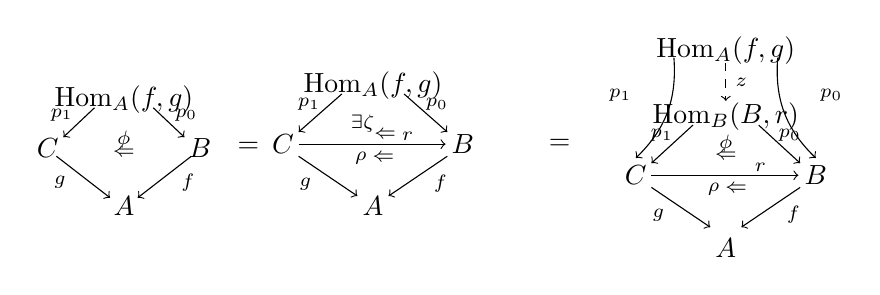
\begin{tikzpicture}[x=1.25em,y=1.25em,baseline=(current bounding box.center)]
  \node (hom) at (0,2.2) {$\mathrm{Hom}_A(f,g)$};
  \node (c) at (-2.2,0.8) {$C$};
  \node (b) at (2.2,0.8) {$B$};
  \node (a) at (0,-0.9) {$A$};
  \draw[->] (-0.85,1.95) -- (-1.75,1.1);
  \node at (-1.8,1.75) {$\scriptstyle p_{1}$};
  \draw[->] (0.85,1.95) -- (1.75,1.1);
  \node at (1.8,1.75) {$\scriptstyle p_{0}$};
  \node at (0,1.02) {$\scriptstyle\phi$};
  \node at (0,0.64) {$\scriptstyle\Leftarrow$};
  \draw[->] (-1.95,0.55) -- (-0.4,-0.65);
  \node at (-1.85,-0.2) {$\scriptstyle g$};
  \draw[->] (1.95,0.55) -- (0.4,-0.65);
  \node at (1.85,-0.2) {$\scriptstyle f$};
  \node at (3.6,0.8) {$=$};
  \begin{scope}[shift={(7.2,0.9)}]
  \node (hom) at (0,1.7) {$\mathrm{Hom}_A(f,g)$};
  \node (c) at (-2.6,0) {$C$};
  \node (b) at (2.6,0) {$B$};
  \node (a) at (0,-1.8) {$A$};
  \draw[->] (-0.9,1.45) -- (-2.15,0.35);
  \node at (-1.85,1.15) {$\scriptstyle p_{1}$};
  \draw[->] (0.9,1.45) -- (2.15,0.35);
  \node at (1.85,1.15) {$\scriptstyle p_{0}$};
  \node at (-0.3,0.6) {$\scriptstyle\exists\zeta$};
  \node at (0.35,0.26) {$\scriptstyle\Leftarrow$};
  \draw[->] (-2.15,0) -- (2.1,0);
  \node at (1.0,0.22) {$\scriptstyle r$};
  \node at (-0.35,-0.4) {$\scriptstyle\rho$};
  \node at (0.3,-0.4) {$\scriptstyle\Leftarrow$};
  \draw[->] (-2.15,-0.35) -- (-0.45,-1.5);
  \node at (-1.95,-1.15) {$\scriptstyle g$};
  \draw[->] (2.15,-0.35) -- (0.45,-1.5);
  \node at (1.95,-1.15) {$\scriptstyle f$};
  \end{scope}
  \node at (12.6,0.9) {$=$};
  \begin{scope}[shift={(17.4,0)}]
  \node (homA) at (0,3.6) {$\mathrm{Hom}_A(f,g)$};
  \node (homB) at (0,1.7) {$\mathrm{Hom}_B(B,r)$};
  \draw[->,dashed] (0,3.25) -- (0,2.15);
  \node at (0.45,2.7) {$\scriptstyle z$};
  \draw[->] (-1.5,3.4) to[bend left=25] (-2.6,0.5);
  \node at (-3.05,2.3) {$\scriptstyle p_{1}$};
  \draw[->] (1.5,3.4) to[bend right=25] (2.6,0.5);
  \node at (3.05,2.3) {$\scriptstyle p_{0}$};
  \node (c) at (-2.6,0) {$C$};
  \node (b) at (2.6,0) {$B$};
  \draw[->] (-0.95,1.45) -- (-2.15,0.35);
  \node at (-1.85,1.15) {$\scriptstyle p_{1}$};
  \draw[->] (0.95,1.45) -- (2.15,0.35);
  \node at (1.85,1.15) {$\scriptstyle p_{0}$};
  \node at (0,0.9) {$\scriptstyle\phi$};
  \node at (0,0.56) {$\scriptstyle\Leftarrow$};
  \draw[->] (-2.15,0) -- (2.1,0);
  \node at (1.0,0.22) {$\scriptstyle r$};
  \node at (-0.35,-0.4) {$\scriptstyle\rho$};
  \node at (0.3,-0.4) {$\scriptstyle\Leftarrow$};
  \draw[->] (-2.15,-0.35) -- (-0.45,-1.5);
  \node at (-1.95,-1.15) {$\scriptstyle g$};
  \draw[->] (2.15,-0.35) -- (0.45,-1.5);
  \node at (1.95,-1.15) {$\scriptstyle f$};
  \node (a) at (0,-2.1) {$A$};
  \end{scope}
\end{tikzpicture}
\end{rveq}
由\trOneCellInduction{}，\trNaturalTransformation{} $\zeta$ 穿过 $r$ 的右\trCommaCone{}作因子分解，如上中所示。%
把 \eqref{eq:absrl-induced-map} 代入上右图的底部，可见 $yz\colon\mathrm{Hom}_A(f,g)\to\mathrm{Hom}_A(f,g)$ 是一个把 $\mathrm{Hom}_A(f,g)$ 的\trCommaCone{}穿过其自身的\trFunctor{}。%
应用命题 3.4.7 的\trUniversalProperty{}，即得：在 $C\times B$ 上存在\trFiberedIsomorphism{}%
$yz\cong\mathrm{id}_{\mathrm{Hom}_A(f,g)}$。

为证 $zy\cong\mathrm{id}_{\mathrm{Hom}_B(B,r)}$，类似地论证 $r$ 的右\trCommaCone{}沿 $zy$ %
限制到自身便已足够。既然 $(r,\rho)$ 是绝对右提升，验证在下方与 $\rho$ 粘贴之后%
$\phi zy=\phi$ 即已足够。但现在把 \eqref{eq:cone-factorization} 与 %
\eqref{eq:absrl-induced-map} 中诸等式的顺序反过来，我们有
\begin{center}
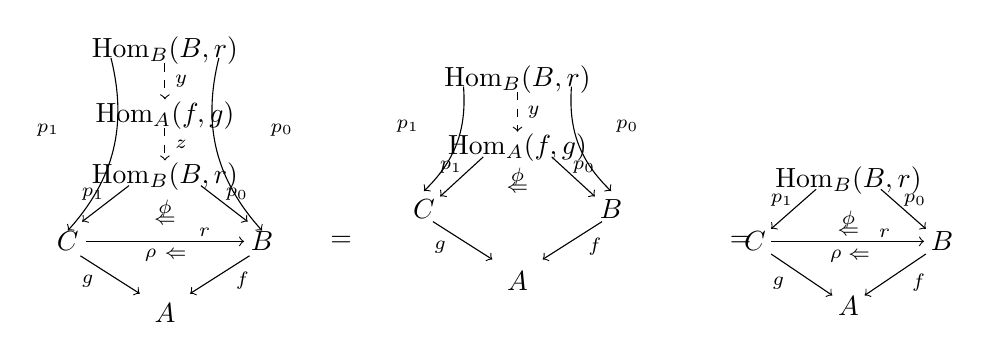
\begin{tikzpicture}[x=1.3em,y=1.3em]
  \node (t1) at (0,4.4) {$\mathrm{Hom}_B(B,r)$};
  \node (t2) at (0,2.6) {$\mathrm{Hom}_A(f,g)$};
  \draw[->,dashed] (0,4.05) -- (0,3.05);
  \node at (0.45,3.55) {$\scriptstyle y$};
  \node (t3) at (0,0.9) {$\mathrm{Hom}_B(B,r)$};
  \draw[->,dashed] (0,2.25) -- (0,1.35);
  \node at (0.45,1.8) {$\scriptstyle z$};
  \draw[->] (-1.5,4.2) to[bend left=28] (-2.7,-0.6);
  \node at (-3.25,2.2) {$\scriptstyle p_{1}$};
  \draw[->] (1.5,4.2) to[bend right=28] (2.7,-0.6);
  \node at (3.25,2.2) {$\scriptstyle p_{0}$};
  \draw[->] (-1.0,0.65) -- (-2.3,-0.35);
  \node at (-2.0,0.4) {$\scriptstyle p_{1}$};
  \draw[->] (1.0,0.65) -- (2.3,-0.35);
  \node at (2.0,0.4) {$\scriptstyle p_{0}$};
  \node at (0,0.0) {$\scriptstyle\phi$};
  \node at (0,-0.34) {$\scriptstyle\Leftarrow$};
  \node (cb) at (-2.7,-0.9) {$C$};
  \node (br) at (2.7,-0.9) {$B$};
  \draw[->] (-2.2,-0.9) -- (2.2,-0.9);
  \node at (1.1,-0.66) {$\scriptstyle r$};
  \node at (-0.4,-1.28) {$\scriptstyle\rho$};
  \node at (0.3,-1.28) {$\scriptstyle\Leftarrow$};
  \draw[->] (-2.35,-1.3) -- (-0.7,-2.35);
  \node at (-2.15,-2.0) {$\scriptstyle g$};
  \draw[->] (2.35,-1.3) -- (0.7,-2.35);
  \node at (2.15,-2.0) {$\scriptstyle f$};
  \node (a) at (0,-2.9) {$A$};
  \node at (4.9,-0.9) {$=$};
  \begin{scope}[shift={(9.8,0)}]
  \node (homB) at (0,3.6) {$\mathrm{Hom}_B(B,r)$};
  \node (homA) at (0,1.7) {$\mathrm{Hom}_A(f,g)$};
  \draw[->,dashed] (0,3.25) -- (0,2.15);
  \node at (0.45,2.7) {$\scriptstyle y$};
  \draw[->] (-1.5,3.4) to[bend left=25] (-2.6,0.5);
  \node at (-3.05,2.3) {$\scriptstyle p_{1}$};
  \draw[->] (1.5,3.4) to[bend right=25] (2.6,0.5);
  \node at (3.05,2.3) {$\scriptstyle p_{0}$};
  \node (c) at (-2.6,0) {$C$};
  \node (b) at (2.6,0) {$B$};
  \draw[->] (-0.95,1.45) -- (-2.15,0.35);
  \node at (-1.85,1.15) {$\scriptstyle p_{1}$};
  \draw[->] (0.95,1.45) -- (2.15,0.35);
  \node at (1.85,1.15) {$\scriptstyle p_{0}$};
  \node at (0,0.9) {$\scriptstyle\phi$};
  \node at (0,0.56) {$\scriptstyle\Leftarrow$};
  \draw[->] (-2.35,-0.35) -- (-0.7,-1.4);
  \node at (-2.15,-1.05) {$\scriptstyle g$};
  \draw[->] (2.35,-0.35) -- (0.7,-1.4);
  \node at (2.15,-1.05) {$\scriptstyle f$};
  \node (a) at (0,-2.0) {$A$};
  \end{scope}
  \node at (16.0,-0.9) {$=$};
  \begin{scope}[shift={(19.0,-0.9)}]
  \node (hom) at (0,1.7) {$\mathrm{Hom}_B(B,r)$};
  \node (c) at (-2.6,0) {$C$};
  \node (b) at (2.6,0) {$B$};
  \node (a) at (0,-1.8) {$A$};
  \draw[->] (-0.9,1.45) -- (-2.15,0.35);
  \node at (-1.85,1.15) {$\scriptstyle p_{1}$};
  \draw[->] (0.9,1.45) -- (2.15,0.35);
  \node at (1.85,1.15) {$\scriptstyle p_{0}$};
  \node at (0,0.6) {$\scriptstyle\phi$};
  \node at (0,0.26) {$\scriptstyle\Leftarrow$};
  \draw[->] (-2.15,0) -- (2.1,0);
  \node at (1.0,0.22) {$\scriptstyle r$};
  \node at (-0.35,-0.4) {$\scriptstyle\rho$};
  \node at (0.3,-0.4) {$\scriptstyle\Leftarrow$};
  \draw[->] (-2.15,-0.35) -- (-0.45,-1.5);
  \node at (-1.95,-1.15) {$\scriptstyle g$};
  \draw[->] (2.15,-0.35) -- (0.45,-1.5);
  \node at (1.95,-1.15) {$\scriptstyle f$};
  \end{scope}
\end{tikzpicture}
\end{center}
这正是所要证明的。于是可见：若 $(r,\rho)$ 是 $g$ 穿过 $f$ 的绝对右提升，则诱导映射 %
\eqref{eq:absrl-induced-map} 定义一个\trFiberedEquivalence{} $\mathrm{Hom}_B(B,r)\simeq\mathrm{Hom}_A(f,g)$。

现在反过来，设 \eqref{eq:absrl-induced-map} 所定义的\trFunctor{} $y$ 是一个%
\trFiberedEquivalence{}，我们来论证 $(r,\rho)$ 是 $g$ 穿过 $f$ 的绝对右提升。由命题 3.4.11，%
\eqref{eq:absrl-induced-map} 中等式左侧所示的\trNaturalTransformation{}从 $\mathrm{Hom}_A(f,g)$ 处继承%
\trCommaCone{}的弱\trUniversalProperty{}。于是命题 3.4.7 供给如下左所示的双射
\begin{center}
\begin{tikzpicture}[x=1.4em,y=1.4em]
  \node at (0,0) {%
  $\left\{\vcenter{\hbox{\begin{tikzpicture}[x=1.3em,y=1.3em]
    \node (x) at (0,2.2) {$X$};
    \node (c) at (-1.9,0.8) {$C$};
    \node (b) at (1.9,0.8) {$B$};
    \node (a) at (0,-1.0) {$A$};
    \draw[->] (-0.5,1.95) -- (-1.5,1.1);
    \node at (-1.5,1.75) {$\scriptstyle c$};
    \draw[->] (0.5,1.95) -- (1.5,1.1);
    \node at (1.5,1.75) {$\scriptstyle b$};
    \node at (0,1.0) {$\scriptstyle\alpha$};
    \node at (0,0.66) {$\scriptstyle\Leftarrow$};
    \draw[->] (-1.65,0.55) -- (-0.35,-0.75);
    \node at (-1.6,-0.35) {$\scriptstyle g$};
    \draw[->] (1.65,0.55) -- (0.35,-0.75);
    \node at (1.6,-0.35) {$\scriptstyle f$};
  \end{tikzpicture}}}\right\}$};
  \node at (3.6,0) {$\longleftrightarrow$};
  \node at (7.6,0) {%
  $\left\{\vcenter{\hbox{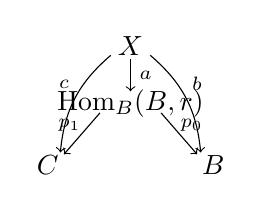
\begin{tikzpicture}[x=1.3em,y=1.3em]
    \node (x) at (0,2.4) {$X$};
    \draw[->] (0,2.05) -- (0,1.15);
    \node at (0.42,1.6) {$\scriptstyle a$};
    \node (hom) at (0,0.8) {$\mathrm{Hom}_B(B,r)$};
    \node (c) at (-2.3,-0.9) {$C$};
    \node (b) at (2.3,-0.9) {$B$};
    \draw[->] (-0.55,2.15) to[bend right=22] (-1.95,-0.55);
    \node at (-1.85,1.35) {$\scriptstyle c$};
    \draw[->] (0.55,2.15) to[bend left=22] (1.95,-0.55);
    \node at (1.85,1.35) {$\scriptstyle b$};
    \draw[->] (-0.85,0.55) -- (-1.85,-0.6);
    \node at (-1.7,0.2) {$\scriptstyle p_{1}$};
    \draw[->] (0.85,0.55) -- (1.85,-0.6);
    \node at (1.7,0.2) {$\scriptstyle p_{0}$};
  \end{tikzpicture}}}\right\}_{/\cong}$};
  \node at (11.6,0) {$\longleftrightarrow$};
  \node at (15.0,0) {%
  $\left\{\vcenter{\hbox{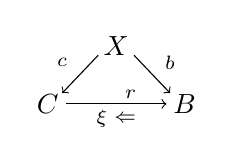
\begin{tikzpicture}[x=1.3em,y=1.3em]
    \node (x) at (0,2.2) {$X$};
    \node (c) at (-1.9,0.6) {$C$};
    \node (b) at (1.9,0.6) {$B$};
    \draw[->] (-0.5,1.95) -- (-1.5,0.9);
    \node at (-1.5,1.75) {$\scriptstyle c$};
    \draw[->] (0.5,1.95) -- (1.5,0.9);
    \node at (1.5,1.75) {$\scriptstyle b$};
    \draw[->] (-1.4,0.6) -- (1.4,0.6);
    \node at (0.4,0.86) {$\scriptstyle r$};
    \node at (-0.4,0.2) {$\scriptstyle\xi$};
    \node at (0.25,0.2) {$\scriptstyle\Leftarrow$};
  \end{tikzpicture}}}\right\}$};
\end{tikzpicture}
\end{center}
——它在\trCospan{}之上的 2-\trCell{}与\trSpan{}映射的\trFiberedIsomorphism{}类之间建立对应，%
其中从中央到左边的实现方式是与 \eqref{eq:absrl-induced-map} 中央处的 2-\trCell{}%
$\rho p_{1}\colon fp_{1}\Rightarrow gp_{1}$ 作\trWhiskering{}。命题 3.4.7 也适用于 %
$r\colon C\to B$ 之上的右\trCommaCone{} $\phi$，给出第二个双射——如上中右所示，居于同样一批%
\trSpan{}映射的\trFiberedIsomorphism{}类与\trCospan{} $C\xrightarrow{\;r\;}B$ 之上的%
2-\trCell{}之间。第二个双射从中央到右边的实现方式是与右\trCommaCone{} $\phi\colon p_{0}\Rightarrow rp_{1}$ %
作粘贴。把二者组合起来便得到：右边所示的 2-\trCell{}与左边所示的 2-\trCell{}之间%
的一个双射，其实现方式为与 $\rho$ 作粘贴——这恰好就是刻划绝对右提升图表的那个%
\trUniversalProperty{}。
\end{proof}

作为该结果的一个特殊情形：

\begin{corollary}\label{cor:fully-faithful}
以下诸条等价，且它们定义了\trInfinityCategory{}之间的\trFunctor{} $f\colon A\to B$ %
何时是\textbf{\trFullyFaithful}（fully faithful）：
\begin{enumerate}[label=(\roman*)]
\item 恒同定义一个绝对右提升图表：
\begin{center}
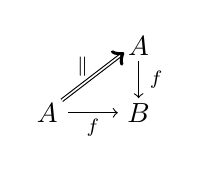
\begin{tikzpicture}[x=1.5em,y=1.5em]
  \node (a1) at (2.2,1.6) {$A$};
  \node (a2) at (0,0) {$A$};
  \node (b) at (2.2,0) {$B$};
  \draw[double,->] (0.35,0.3) -- (1.85,1.45);
  \node at (0.85,1.1) {$\scriptstyle\parallel$};
  \draw[->] (2.2,1.25) -- (2.2,0.35);
  \node at (2.62,0.8) {$\scriptstyle f$};
  \draw[->] (0.5,0) -- (1.7,0);
  \node at (1.1,-0.36) {$\scriptstyle f$};
\end{tikzpicture}
\end{center}
\item 恒同定义一个绝对左提升图表：
\begin{center}
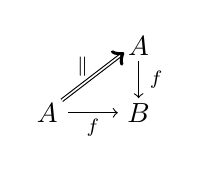
\begin{tikzpicture}[x=1.5em,y=1.5em]
  \node (a1) at (2.2,1.6) {$A$};
  \node (a2) at (0,0) {$A$};
  \node (b) at (2.2,0) {$B$};
  \draw[double,->] (0.35,0.3) -- (1.85,1.45);
  \node at (0.85,1.1) {$\scriptstyle\parallel$};
  \draw[->] (2.2,1.25) -- (2.2,0.35);
  \node at (2.62,0.8) {$\scriptstyle f$};
  \draw[->] (0.5,0) -- (1.7,0);
  \node at (1.1,-0.36) {$\scriptstyle f$};
\end{tikzpicture}
\end{center}
\item 对任何\trInfinityCategory{} $X$，诱导\trFunctor
\[
f_{*}\colon\mathrm{hFun}(X,A)\to\mathrm{hFun}(X,B)
\]
是一个 1-\trCategory{}之间的\trFullyFaithful{}\trFunctor{}。
\item 由恒同 2-\trCell{} $\mathrm{id}_f$ 所诱导的\trFunctor{}定义一个\trFiberedEquivalence{}%
$A^{2}\simeq_{A\times A}\mathrm{Hom}_B(f,f)$。
\begin{center}
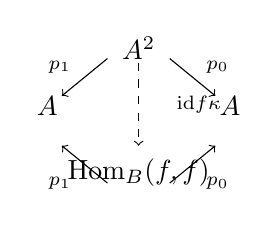
\begin{tikzpicture}[x=1.5em,y=1.5em]
  \node (a2) at (0,2.2) {$A^{2}$};
  \node (al) at (-2.2,0.8) {$A$};
  \node (ar) at (2.2,0.8) {$A$};
  \node (hom) at (0,-0.8) {$\mathrm{Hom}_B(f,f)$};
  \draw[->] (-0.75,1.95) -- (-1.85,1.05);
  \node at (-1.9,1.75) {$\scriptstyle p_{1}$};
  \draw[->] (0.75,1.95) -- (1.85,1.05);
  \node at (1.9,1.75) {$\scriptstyle p_{0}$};
  \draw[->,dashed] (0,1.85) -- (0,-0.15);
  \node at (1.45,0.85) {$\scriptstyle\mathrm{id}\qcor{f\kappa}$};
  \draw[->] (-0.75,-1.05) -- (-1.85,-0.15);
  \node at (-1.9,-1.05) {$\scriptstyle p_{1}$};
  \draw[->] (0.75,-1.05) -- (1.85,-0.15);
  \node at (1.9,-1.05) {$\scriptstyle p_{0}$};
\end{tikzpicture}
\end{center}
\end{enumerate}
\end{corollary}

\begin{proof}
陈述 (iii) 是 (i) 与 (ii) 之含义的展开。\cref{thm:absrl-equivalence}特殊化后证明 %
(i)$\Leftrightarrow$(iv)，或对偶地 (ii)$\Leftrightarrow$(iv)。
\end{proof}

用\trInfinityCategory{}之间的一个\trFullyFaithful{}\trFunctor{}作\trPostComposition{}会在%
\trHomotopyTwoCategory{}中诱导\trHomCategory{}之间的\trFullyFaithful{}\trFunctor——特别地诱导%
\trHomotopyCategory{}之间的\trFullyFaithful{}\trFunctor{}（见第 1 章中的定义 1.4.11），这并不令人%
惊讶。较不显然的是：这一条件竟强到足以捕捉∞-范畴论的全忠实性概念，尽管可以肯定，%
仅仅要求\trFunctor{} $\mathrm{h}f\colon\mathrm{h}A\to\mathrm{h}B$ \trFullyFaithful{}是不够的。%
条件 (iii) 出人意料的力量在于：其陈述对 $A$ 的所有\trGeneralizedElement{}%
$a\colon X\to A$ 做了全称量化，而 $\mathrm{h}A$ 的对象则局限于诸\trElement{}%
$a\colon\qcOne\to A$。这为我们在\trHomotopyTwoCategory{}中所做的工作提供了追溯性的辩护。

\cref{thm:absrl-equivalence}还有另一条重要推论，在第 2 章中的命题 2.4.7 的证明中%
曾被引用。

\begin{corollary}\label{cor:cosmological-absrl}
\trCosmologicalFunctor{}保持绝对提升图表。
\end{corollary}

\begin{proof}
考察一个\trCosmologicalFunctor{} $F\colon\mathcal{K}\to\mathcal{L}$ 连同 $\mathcal{K}$ %
中的一个绝对右提升图表：
\begin{center}
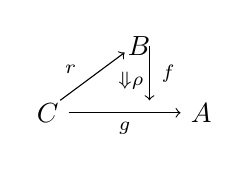
\begin{tikzpicture}[x=1.5em,y=1.5em]
  \node (b) at (2.2,1.6) {$B$};
  \node (c) at (0,0) {$C$};
  \node (a) at (3.7,0) {$A$};
  \draw[->] (0.3,0.3) -- (1.85,1.45);
  \node at (0.55,1.05) {$\scriptstyle r$};
  \node at (2.0,0.78) {$\scriptstyle\Downarrow\rho$};
  \draw[->] (2.45,1.6) -- (2.45,0.3);
  \node at (2.9,0.95) {$\scriptstyle f$};
  \draw[->] (0.5,0) -- (3.2,0);
  \node at (1.85,-0.36) {$\scriptstyle g$};
\end{tikzpicture}
\end{center}
由\cref{thm:absrl-equivalence}，\eqref{eq:absrl-induced-map} 的诱导\trFunctor{}定义一个%
\trFiberedEquivalence{} $y\colon\mathrm{Hom}_B(B,r)\to\mathrm{Hom}_A(f,g)$——居于%
$C\times B$ 之上。由于\trCosmologicalFunctor{}保持式 (3.4.2) 中的\trSimplicial\trLimit{}%
与\trIsofibration{}，$F$ 把 $y$ 带为一个\trFunctor{} %
$Fy\colon\mathrm{Hom}_{FB}(FB,Fr)\to\mathrm{Hom}_{FA}(Ff,Fg)$——居于 $FC\times FB$ 之上。由第 1 章中的引理 1.3.2，%
该\trFunctor{}仍是\trFiberedEquivalence{}。由于\trCosmologicalFunctor{}定义 2-\trFunctor{}，%
该\trFunctor{}满足 $\mathcal{L}$ 中的一个粘贴等式
\begin{center}
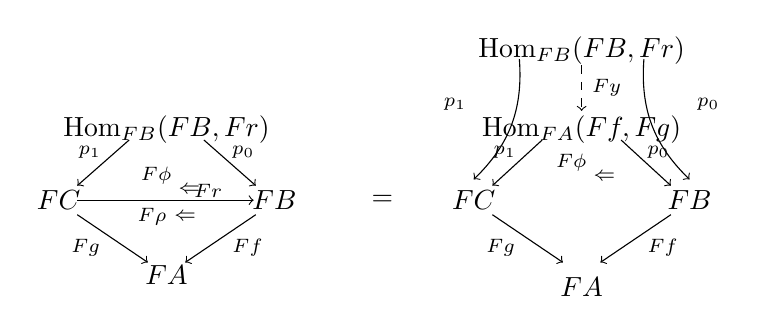
\begin{tikzpicture}[x=1.5em,y=1.5em]
  \node (hom) at (0,1.7) {$\mathrm{Hom}_{FB}(FB,Fr)$};
  \node (c) at (-2.6,0) {$FC$};
  \node (b) at (2.6,0) {$FB$};
  \node (a) at (0,-1.8) {$FA$};
  \draw[->] (-0.9,1.45) -- (-2.15,0.35);
  \node at (-1.85,1.15) {$\scriptstyle p_{1}$};
  \draw[->] (0.9,1.45) -- (2.15,0.35);
  \node at (1.85,1.15) {$\scriptstyle p_{0}$};
  \node at (-0.25,0.6) {$\scriptstyle F\phi$};
  \node at (0.55,0.26) {$\scriptstyle\Leftarrow$};
  \draw[->] (-2.15,0) -- (2.1,0);
  \node at (1.0,0.22) {$\scriptstyle Fr$};
  \node at (-0.35,-0.4) {$\scriptstyle F\rho$};
  \node at (0.45,-0.4) {$\scriptstyle\Leftarrow$};
  \draw[->] (-2.15,-0.35) -- (-0.45,-1.5);
  \node at (-1.95,-1.15) {$\scriptstyle Fg$};
  \draw[->] (2.15,-0.35) -- (0.45,-1.5);
  \node at (1.95,-1.15) {$\scriptstyle Ff$};
  \node at (5.2,0) {$=$};
  \begin{scope}[shift={(10.0,0)}]
  \node (homB) at (0,3.6) {$\mathrm{Hom}_{FB}(FB,Fr)$};
  \node (homA) at (0,1.7) {$\mathrm{Hom}_{FA}(Ff,Fg)$};
  \draw[->,dashed] (0,3.25) -- (0,2.15);
  \node at (0.6,2.7) {$\scriptstyle Fy$};
  \draw[->] (-1.5,3.4) to[bend left=25] (-2.6,0.5);
  \node at (-3.05,2.3) {$\scriptstyle p_{1}$};
  \draw[->] (1.5,3.4) to[bend right=25] (2.6,0.5);
  \node at (3.05,2.3) {$\scriptstyle p_{0}$};
  \node (c) at (-2.6,0) {$FC$};
  \node (b) at (2.6,0) {$FB$};
  \draw[->] (-0.95,1.45) -- (-2.15,0.35);
  \node at (-1.85,1.15) {$\scriptstyle p_{1}$};
  \draw[->] (0.95,1.45) -- (2.15,0.35);
  \node at (1.85,1.15) {$\scriptstyle p_{0}$};
  \node at (-0.25,0.9) {$\scriptstyle F\phi$};
  \node at (0.55,0.56) {$\scriptstyle\Leftarrow$};
  \draw[->] (-2.15,-0.35) -- (-0.45,-1.5);
  \node at (-1.95,-1.15) {$\scriptstyle Fg$};
  \draw[->] (2.15,-0.35) -- (0.45,-1.5);
  \node at (1.95,-1.15) {$\scriptstyle Ff$};
  \node (a) at (0,-2.1) {$FA$};
  \end{scope}
\end{tikzpicture}
\end{center}
由\cref{thm:absrl-equivalence}，这一\trFiberedEquivalence{}见证了下述图表
\begin{center}
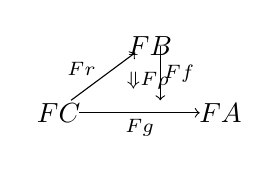
\begin{tikzpicture}[x=1.5em,y=1.5em]
  \node (b) at (2.2,1.6) {$FB$};
  \node (c) at (0,0) {$FC$};
  \node (a) at (3.9,0) {$FA$};
  \draw[->] (0.3,0.3) -- (1.85,1.45);
  \node at (0.55,1.05) {$\scriptstyle Fr$};
  \node at (2.15,0.78) {$\scriptstyle\Downarrow F\rho$};
  \draw[->] (2.45,1.6) -- (2.45,0.3);
  \node at (2.9,0.95) {$\scriptstyle Ff$};
  \draw[->] (0.5,0) -- (3.4,0);
  \node at (1.95,-0.36) {$\scriptstyle Fg$};
\end{tikzpicture}
\end{center}
定义 $\mathcal{L}$ 中的一个绝对右提升图表。
\end{proof}

在证明\cref{thm:absrl-equivalence}之后，我们的当务之急是把该定理强化为：
纤维化等价 $\mathrm{Hom}_B(B,r)\simeq_{C\times B}\mathrm{Hom}_A(f,g)$
蕴含 $r\colon C\to B$ 定义 $g$ 穿过 $f$ 的一个绝对右提升——
而无须先前指定 2-\trCell{} $\rho\colon fr\Rightarrow g$。

\begin{theorem}\label{thm:trio-bijection}
给定三元\trFunctor{}组 $r\colon C\to B$、$f\colon B\to A$ 与 $g\colon C\to A$，%
在下左所示的\trNaturalTransformation{}与下右所示的\trSpan{}映射的\trFiberedIsomorphism{}类之间
\begin{center}
\begin{tikzpicture}[x=1.4em,y=1.4em]
  \node at (0,0) {%
  $\left\{\vcenter{\hbox{\begin{tikzpicture}[x=1.3em,y=1.3em]
    \node (b) at (0.9,1.6) {$B$};
    \node (c) at (-1.4,0) {$C$};
    \node (a) at (2.4,0) {$A$};
    \draw[->] (-1.1,0.3) -- (0.55,1.45);
    \node at (-0.85,1.05) {$\scriptstyle r$};
    \node at (0.7,0.78) {$\scriptstyle\Downarrow\rho$};
    \draw[->] (1.15,1.6) -- (1.15,0.3);
    \node at (1.6,0.95) {$\scriptstyle f$};
    \draw[->] (-1.0,0) -- (1.9,0);
    \node at (0.45,-0.36) {$\scriptstyle g$};
  \end{tikzpicture}}}\right\}$};
  \node at (4.4,0.6) {$\longleftrightarrow$};
  \node at (10.6,0.6) {%
  $\left\{\vcenter{\hbox{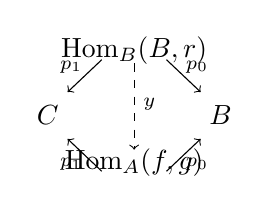
\begin{tikzpicture}[x=1.3em,y=1.3em]
    \node (homB) at (0,2.4) {$\mathrm{Hom}_B(B,r)$};
    \draw[->] (-0.9,2.15) -- (-1.85,1.25);
    \node at (-1.75,1.95) {$\scriptstyle p_{1}$};
    \draw[->] (0.9,2.15) -- (1.85,1.25);
    \node at (1.75,1.95) {$\scriptstyle p_{0}$};
    \draw[->,dashed] (0,2.05) -- (0,-0.35);
    \node at (0.42,0.9) {$\scriptstyle y$};
    \node (homA) at (0,-0.7) {$\mathrm{Hom}_A(f,g)$};
    \node (c) at (-2.4,0.6) {$C$};
    \node (b) at (2.4,0.6) {$B$};
    \draw[->] (-0.9,-0.95) -- (-1.85,-0.05);
    \node at (-1.75,-0.75) {$\scriptstyle p_{1}$};
    \draw[->] (0.9,-0.95) -- (1.85,-0.05);
    \node at (1.75,-0.75) {$\scriptstyle p_{0}$};
  \end{tikzpicture}}}\right\}_{/\cong}$};
\end{tikzpicture}
\end{center}
存在一个双射；该双射由与 $r$ 之上的右\trCommaCone{}作粘贴、再应用\trOneCellInduction{}穿过%
$\mathrm{Hom}_A(f,g)$ 的\trCommaCone{}作因子分解而构造。
\begin{center}
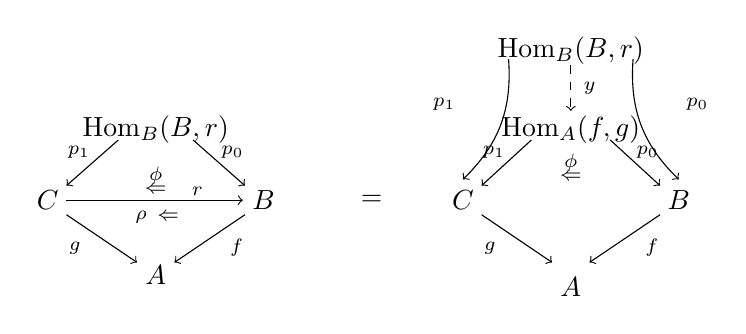
\begin{tikzpicture}[x=1.5em,y=1.5em]
  \node (hom) at (0,1.7) {$\mathrm{Hom}_B(B,r)$};
  \node (c) at (-2.6,0) {$C$};
  \node (b) at (2.6,0) {$B$};
  \node (a) at (0,-1.8) {$A$};
  \draw[->] (-0.9,1.45) -- (-2.15,0.35);
  \node at (-1.85,1.15) {$\scriptstyle p_{1}$};
  \draw[->] (0.9,1.45) -- (2.15,0.35);
  \node at (1.85,1.15) {$\scriptstyle p_{0}$};
  \node at (0,0.6) {$\scriptstyle\phi$};
  \node at (0,0.26) {$\scriptstyle\Leftarrow$};
  \draw[->] (-2.15,0) -- (2.1,0);
  \node at (1.0,0.22) {$\scriptstyle r$};
  \node at (-0.35,-0.4) {$\scriptstyle\rho$};
  \node at (0.3,-0.4) {$\scriptstyle\Leftarrow$};
  \draw[->] (-2.15,-0.35) -- (-0.45,-1.5);
  \node at (-1.95,-1.15) {$\scriptstyle g$};
  \draw[->] (2.15,-0.35) -- (0.45,-1.5);
  \node at (1.95,-1.15) {$\scriptstyle f$};
  \node at (5.2,0) {$=$};
  \begin{scope}[shift={(10.0,0)}]
  \node (homB) at (0,3.6) {$\mathrm{Hom}_B(B,r)$};
  \node (homA) at (0,1.7) {$\mathrm{Hom}_A(f,g)$};
  \draw[->,dashed] (0,3.25) -- (0,2.15);
  \node at (0.45,2.7) {$\scriptstyle y$};
  \draw[->] (-1.5,3.4) to[bend left=25] (-2.6,0.5);
  \node at (-3.05,2.3) {$\scriptstyle p_{1}$};
  \draw[->] (1.5,3.4) to[bend right=25] (2.6,0.5);
  \node at (3.05,2.3) {$\scriptstyle p_{0}$};
  \node (c) at (-2.6,0) {$C$};
  \node (b) at (2.6,0) {$B$};
  \draw[->] (-0.95,1.45) -- (-2.15,0.35);
  \node at (-1.85,1.15) {$\scriptstyle p_{1}$};
  \draw[->] (0.95,1.45) -- (2.15,0.35);
  \node at (1.85,1.15) {$\scriptstyle p_{0}$};
  \node at (0,0.9) {$\scriptstyle\phi$};
  \node at (0,0.56) {$\scriptstyle\Leftarrow$};
  \draw[->] (-2.15,-0.35) -- (-0.45,-1.5);
  \node at (-1.95,-1.15) {$\scriptstyle g$};
  \draw[->] (2.15,-0.35) -- (0.45,-1.5);
  \node at (1.95,-1.15) {$\scriptstyle f$};
  \node (a) at (0,-2.1) {$A$};
  \end{scope}
\end{tikzpicture}
\end{center}
此外，\trNaturalTransformation{} $\rho\colon fr\Rightarrow g$ 把 $r$ 展示为 $g$ 穿过 $f$ 的绝对右提升，%
当且仅当相应映射 $y\colon\mathrm{Hom}_B(B,r)\to\mathrm{Hom}_A(f,g)$ 是一个\trEquivalence{}。
\end{theorem}

第二款即\cref{thm:absrl-equivalence}的陈述，故只剩第一款待证。我们通过展示所宣称构造%
的逆来证明它是一个双射；该逆的构造涉及一条颇为神秘的引理，其意义将%
逐渐显明。

\begin{lemma}\label{lem:right-adjoint-right-inverse}
对任何\trFunctor{} $f\colon A\to B$，其右表示的\textbf{余定义域投影函子}（codomain %
projection functor）$p_{1}\colon\mathrm{Hom}_B(B,f)\twoheadrightarrow A$ 具有一个%
\textbf{\trRightAdjoint\trRightInverse}（right adjoint right inverse）%
\footnote{一个\trFunctor{}具有\trRightAdjoint\trRightInverse{}，当且仅当它是\trCounit{}可逆的一个\trAdjunction{}中的\trLeftAdjoint%
（见 B.4 节）。当原来的\trFunctor{}是\trIsofibration{}时——此处正是这种情形——任何%
\trRightAdjoint\trRightInverse{}\trAdjunction{}都可升级为\trCounit{}为恒同的\trAdjunction{}，而后者又可进一步升级为纤维化\trAdjunction%
（见定义 3.6.5 与引理 3.6.9）。}
$i:=\qcor{\mathrm{id}_f}$——由恒同 2-\trCell{} $\mathrm{id}_f$ 诱导——从而定义了 $A$ %
之上的一个\trAdjunction{}，其\trCounit{}是恒同，其\trUnit{} $\eta\colon\mathrm{id}\Rightarrow ip_{1}$ %
满足条件 $\eta i=\mathrm{id}_i$、$p_{1}\eta=\mathrm{id}_{p_{1}}$ 与 $p_{0}\eta=\phi$。
\begin{center}
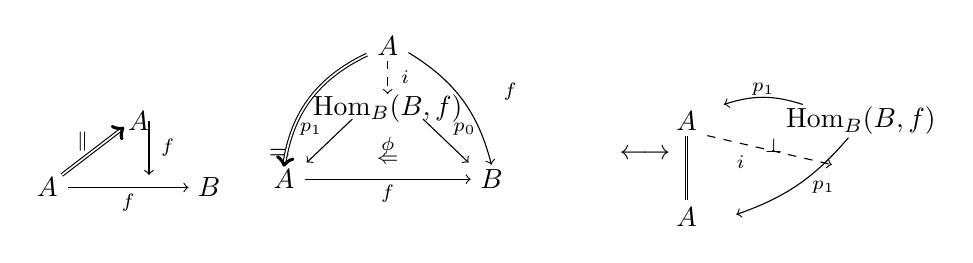
\begin{tikzpicture}[x=1.5em,y=1.5em]
  \node (a1) at (2.2,1.6) {$A$};
  \node (a2) at (0,0) {$A$};
  \node (b) at (3.9,0) {$B$};
  \draw[double,->] (0.35,0.3) -- (1.85,1.45);
  \node at (0.85,1.1) {$\scriptstyle\parallel$};
  \draw[->] (2.45,1.6) -- (2.45,0.3);
  \node at (2.9,0.95) {$\scriptstyle f$};
  \draw[->] (0.5,0) -- (3.4,0);
  \node at (1.95,-0.36) {$\scriptstyle f$};
  \node at (5.6,0.8) {$=$};
  \begin{scope}[shift={(8.2,0)}]
  \node (atop) at (0,3.4) {$A$};
  \draw[->,dashed] (0,3.05) -- (0,2.25);
  \node at (0.42,2.65) {$\scriptstyle i$};
  \node (hom) at (0,1.9) {$\mathrm{Hom}_B(B,f)$};
  \draw[->] (0.5,3.25) to[bend left=22] (2.5,0.55);
  \node at (2.95,2.3) {$\scriptstyle f$};
  \draw[double,->] (-0.5,3.2) to[bend right=28] (-2.5,0.5);
  \node (ab) at (-2.5,0.2) {$A$};
  \node (bb) at (2.5,0.2) {$B$};
  \draw[->] (-0.85,1.65) -- (-1.95,0.6);
  \node at (-1.85,1.4) {$\scriptstyle p_{1}$};
  \draw[->] (0.85,1.65) -- (1.95,0.6);
  \node at (1.85,1.4) {$\scriptstyle p_{0}$};
  \node at (0,1.0) {$\scriptstyle\phi$};
  \node at (0,0.66) {$\scriptstyle\Leftarrow$};
  \draw[->] (-2.0,0.2) -- (2.0,0.2);
  \node at (0,-0.16) {$\scriptstyle f$};
  \end{scope}
  \node at (14.4,0.8) {$\longleftrightarrow$};
  \begin{scope}[shift={(17.2,0)}]
  \node (a1) at (-1.8,1.6) {$A$};
  \node (h) at (2.4,1.6) {$\mathrm{Hom}_B(B,f)$};
  \draw[->] (1.0,2.0) to[bend right=18] (-0.9,2.0);
  \node at (0.05,2.36) {$\scriptstyle p_{1}$};
  \node at (0.3,1.0) {$\scriptstyle\perp$};
  \draw[->,dashed] (-1.3,1.25) -- (1.7,0.55);
  \node at (-0.5,0.6) {$\scriptstyle i$};
  \draw[double] (-1.8,1.25) -- (-1.8,-0.3);
  \node (a2) at (-1.8,-0.7) {$A$};
  \draw[->] (2.1,1.2) to[bend left=15] (-0.6,-0.65);
  \node at (1.5,0.0) {$\scriptstyle p_{1}$};
  \end{scope}
\end{tikzpicture}
\end{center}
\end{lemma}

这条引理在 5.7 节的\trYonedaLemma{}证明中扮演重要角色，它也是以\cref{cor:cheap-yoneda}%
出现的「廉价」版\trYonedaLemma{}的主要成分。

\begin{proof}
这一\trAdjunction{}经由 $f$ 之上的右\trCommaCone{}的弱\trUniversalProperty{}构造。恒同 2-\trCell{}%
$\mathrm{id}_f$ 在 $f$ 之上的右\trCommaCone{}之上诱导一个\trFunctor{} $i:=\qcor{\mathrm{id}_f}$，%
如陈述中所示。注意 $p_{1}i=\mathrm{id}_A$，故我们可以取\trCounit{}为恒同 2-\trCell{}。由于 %
$\phi i=\mathrm{id}_f$，我们有粘贴等式
\begin{center}
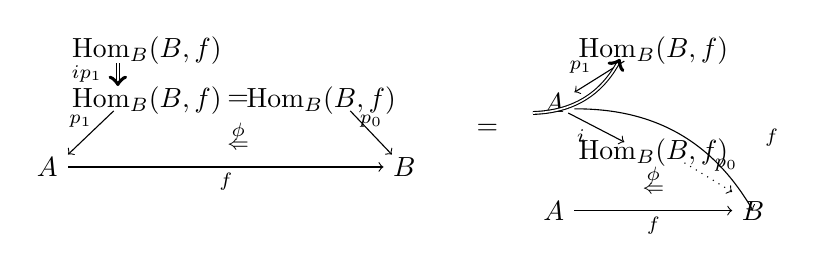
\begin{tikzpicture}[x=1.5em,y=1.5em]
  \node (h1) at (-1.8,3.3) {$\mathrm{Hom}_B(B,f)$};
  \draw[double,->] (-2.5,3.0) -- (-2.5,2.45);
  \node at (-3.25,2.75) {$\scriptstyle ip_{1}$};
  \node (h2) at (-1.8,2.1) {$\mathrm{Hom}_B(B,f)$};
  \node (eq) at (0.4,2.1) {$=$};
  \node (h3) at (2.4,2.1) {$\mathrm{Hom}_B(B,f)$};
  \node (a) at (-4.2,0.5) {$A$};
  \node (b) at (4.4,0.5) {$B$};
  \draw[->] (-2.6,1.85) -- (-3.7,0.8);
  \node at (-3.4,1.6) {$\scriptstyle p_{1}$};
  \draw[->] (3.1,1.85) -- (4.1,0.8);
  \node at (3.6,1.6) {$\scriptstyle p_{0}$};
  \node at (0.4,1.35) {$\scriptstyle\phi$};
  \node at (0.4,1.01) {$\scriptstyle\Leftarrow$};
  \draw[->] (-3.7,0.5) -- (3.9,0.5);
  \node at (0.1,0.14) {$\scriptstyle f$};
  \node at (6.4,1.4) {$=$};
  \begin{scope}[shift={(10.4,0)}]
  \node (H1) at (0,3.3) {$\mathrm{Hom}_B(B,f)$};
  \draw[->] (-0.7,3.05) -- (-1.9,2.3);
  \node at (-1.75,2.9) {$\scriptstyle p_{1}$};
  \node (am) at (-2.4,2.05) {$A$};
  \draw[double,->] (-2.9,1.8) to[bend right=30] (-0.8,3.1);
  \draw[->] (-2.05,1.8) -- (-0.7,1.1);
  \node at (-1.75,1.25) {$\scriptstyle i$};
  \node (H2) at (0,0.85) {$\mathrm{Hom}_B(B,f)$};
  \node at (0,0.3) {$\scriptstyle\phi$};
  \node at (0,-0.04) {$\scriptstyle\Leftarrow$};
  \draw[->,dotted] (0.75,0.6) -- (1.9,-0.1);
  \node at (1.75,0.55) {$\scriptstyle p_{0}$};
  \draw[->] (-1.9,1.9) to[bend left=30] (2.4,-0.55);
  \node at (2.85,1.2) {$\scriptstyle f$};
  \node (a2) at (-2.4,-0.55) {$A$};
  \node (b2) at (2.4,-0.55) {$B$};
  \draw[->] (-1.9,-0.55) -- (1.9,-0.55);
  \node at (0,-0.91) {$\scriptstyle f$};
  \end{scope}
\end{tikzpicture}
\end{center}
它诱导一个 2-\trCell{} $\eta\colon\mathrm{id}\Rightarrow ip_{1}$，其定义等式为 %
$p_{1}\eta=\mathrm{id}_{p_{1}}$ 与 $p_{0}\eta=\phi$。前一条给出一个\trTriangleEqualities{}；%
为得另一条，我们必须验证 $\eta i=\mathrm{id}_i$。由\trTwoCellConservativity{}，$\eta i$ %
是一个\trIsomorphism{}，因为 $p_{1}\eta i=\mathrm{id}_A$ 与 $p_{0}\eta i=\mathrm{id}_f$ %
都\trInvertible{}。由\trWhiskering{}的自然性，我们有
\begin{center}
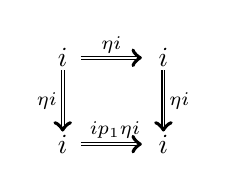
\begin{tikzpicture}[x=1.3em,y=1.3em]
  \node (tl) at (0,1.2) {$i$};
  \node (tr) at (2.8,1.2) {$i$};
  \node (bl) at (0,-1.2) {$i$};
  \node (br) at (2.8,-1.2) {$i$};
  \draw[double,->] (0.5,1.2) -- (2.2,1.2);
  \node at (1.35,1.55) {$\scriptstyle\eta i$};
  \draw[double,->] (0.5,-1.2) -- (2.2,-1.2);
  \node at (1.45,-0.82) {$\scriptstyle ip_{1}\eta i$};
  \draw[double,->] (0,0.85) -- (0,-0.85);
  \node at (-0.44,0) {$\scriptstyle\eta i$};
  \draw[double,->] (2.8,0.85) -- (2.8,-0.85);
  \node at (3.24,0) {$\scriptstyle\eta i$};
\end{tikzpicture}
\end{center}
而由于 $p_{1}\eta=\mathrm{id}_{p_{1}}$，底边是恒同。于是 $\eta i\cdot\eta i=\eta i$，%
又 $\eta i$ 是\trIsomorphism{}，消去即得 $\eta i=\mathrm{id}_i$，如所要证。
\end{proof}

\cref{lem:right-adjoint-right-inverse}的一种诠释最好通过一个特殊情形来揭示：

\begin{corollary}\label{cor:terminal-element}
对任何\trElement{} $b\colon\qcOne\to B$，$b$ 处的恒同在 $\mathrm{Hom}_B(B,b)$ 中%
定义一个\trTerminal{}元素。
\end{corollary}

\begin{proof}
由\cref{lem:right-adjoint-right-inverse}，余定义域投影——在此情形下约化为唯一\trFunctor{}%
$!\colon\mathrm{Hom}_B(B,b)\to\qcOne$——具有由其恒同 2-\trCell{}诱导的一个\trRightAdjoint\trRightInverse{}。%
于是，由第 2 章中的定义 2.2.1，该\trRightAdjoint{}甄别出一个\trTerminal{}元素 %
$\qcor{\mathrm{id}_b}\colon\qcOne\to\mathrm{Hom}_B(B,b)$，对应于\trHomotopyCategory{}%
$\mathrm{h}B$ 中的恒同态射 $\mathrm{id}_b\colon b\to b$。
\end{proof}

\cref{lem:right-adjoint-right-inverse}的一般版本有一个类似的诠释：$\mathrm{id}_f$ %
在「$A$ 之上」的 $\mathrm{Hom}_B(B,f)$ 中——也就是说，在\trSliceInfinityCosmos{}中——诱导一个%
\trTerminal{}元素（见定义 3.6.8 与例 3.6.12）。

\begin{proof}[\cref{thm:trio-bijection}之证]
尚需构造陈述中那个映射的逆：它取\trNaturalTransformation{} $fr\Rightarrow g$，产出居于 $C\times B$ %
之上的诸\trFunctor{} $\mathrm{Hom}_B(B,r)\to\mathrm{Hom}_A(f,g)$ 的一个%
\trFiberedIsomorphism{}类。我们的构造利用\cref{lem:right-adjoint-right-inverse}的%
\trRightAdjoint\trRightInverse{} $i\colon C\to\mathrm{Hom}_B(B,r)$。给定一个\trFunctor{} $\mathrm{Hom}_B(B,r)\to\mathrm{Hom}_A(f,g)$，沿 $i$ 限制，再与 $\mathrm{Hom}_A(f,g)$ 的\trCommaCone{}作粘贴，%
便定义一个\trNaturalTransformation{} $fr\Rightarrow g$。

从\trNaturalTransformation{} $\rho\colon fr\Rightarrow g$ 出发，这两个映射的复合构造出下左所示的\trNaturalTransformation{}
\begin{center}
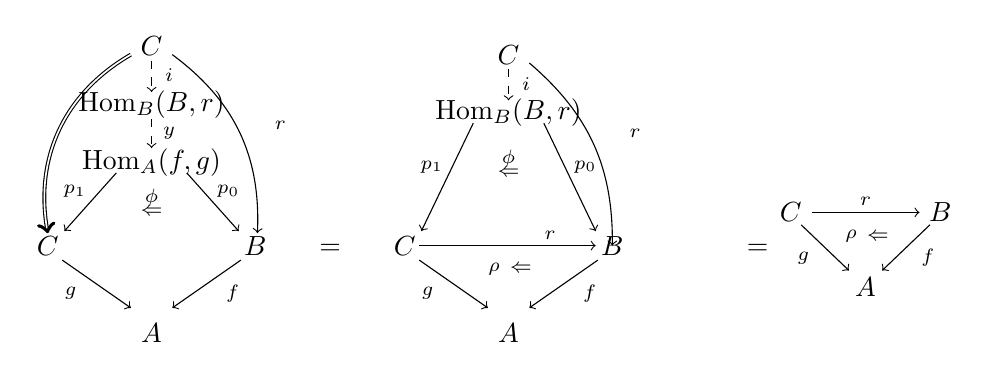
\begin{tikzpicture}[x=1.5em,y=1.5em]
  \node (ctop) at (0,4.6) {$C$};
  \draw[double,->] (-0.5,4.4) to[bend right=35] (-2.5,0.1);
  \draw[->,dashed] (0,4.25) -- (0,3.5);
  \node at (0.42,3.9) {$\scriptstyle i$};
  \node (hb) at (0,3.2) {$\mathrm{Hom}_B(B,r)$};
  \draw[->,dashed] (0,2.85) -- (0,2.15);
  \node at (0.42,2.5) {$\scriptstyle y$};
  \node (ha) at (0,1.8) {$\mathrm{Hom}_A(f,g)$};
  \draw[->] (0.5,4.4) to[bend left=28] (2.55,0.1);
  \node at (3.1,2.7) {$\scriptstyle r$};
  \node (c) at (-2.5,-0.2) {$C$};
  \node (b) at (2.5,-0.2) {$B$};
  \draw[->] (-0.85,1.55) -- (-2.1,0.15);
  \node at (-1.85,1.1) {$\scriptstyle p_{1}$};
  \draw[->] (0.85,1.55) -- (2.1,0.15);
  \node at (1.85,1.1) {$\scriptstyle p_{0}$};
  \node at (0,0.95) {$\scriptstyle\phi$};
  \node at (0,0.61) {$\scriptstyle\Leftarrow$};
  \draw[->] (-2.15,-0.55) -- (-0.5,-1.7);
  \node at (-1.95,-1.35) {$\scriptstyle g$};
  \draw[->] (2.15,-0.55) -- (0.5,-1.7);
  \node at (1.95,-1.35) {$\scriptstyle f$};
  \node (a) at (0,-2.3) {$A$};
  \node at (4.3,-0.3) {$=$};
  \begin{scope}[shift={(8.6,0)}]
  \node (ctop) at (0,4.4) {$C$};
  \draw[->,dashed] (0,4.05) -- (0,3.3);
  \node at (0.42,3.7) {$\scriptstyle i$};
  \draw[->] (0.5,4.2) to[bend left=25] (2.5,-0.2);
  \node at (3.05,2.5) {$\scriptstyle r$};
  \node (hb) at (0,3.0) {$\mathrm{Hom}_B(B,r)$};
  \node (c) at (-2.5,-0.2) {$C$};
  \node (b) at (2.5,-0.2) {$B$};
  \draw[->] (-0.85,2.75) -- (-2.1,0.15);
  \node at (-1.85,1.7) {$\scriptstyle p_{1}$};
  \draw[->] (0.85,2.75) -- (2.1,0.15);
  \node at (1.85,1.7) {$\scriptstyle p_{0}$};
  \node at (0,1.9) {$\scriptstyle\phi$};
  \node at (0,1.56) {$\scriptstyle\Leftarrow$};
  \draw[->] (-2.15,-0.2) -- (2.1,-0.2);
  \node at (1.0,0.04) {$\scriptstyle r$};
  \node at (-0.35,-0.76) {$\scriptstyle\rho$};
  \node at (0.3,-0.76) {$\scriptstyle\Leftarrow$};
  \draw[->] (-2.15,-0.55) -- (-0.5,-1.7);
  \node at (-1.95,-1.35) {$\scriptstyle g$};
  \draw[->] (2.15,-0.55) -- (0.5,-1.7);
  \node at (1.95,-1.35) {$\scriptstyle f$};
  \node (a) at (0,-2.3) {$A$};
  \end{scope}
  \node at (14.6,-0.3) {$=$};
  \begin{scope}[shift={(17.2,-0.3)}]
  \node (c) at (-1.8,0.9) {$C$};
  \node (b) at (1.8,0.9) {$B$};
  \draw[->] (-1.3,0.9) -- (1.3,0.9);
  \node at (0,1.16) {$\scriptstyle r$};
  \node at (-0.35,0.32) {$\scriptstyle\rho$};
  \node at (0.3,0.32) {$\scriptstyle\Leftarrow$};
  \draw[->] (-1.55,0.6) -- (-0.4,-0.5);
  \node at (-1.5,-0.2) {$\scriptstyle g$};
  \draw[->] (1.55,0.6) -- (0.4,-0.5);
  \node at (1.5,-0.2) {$\scriptstyle f$};
  \node (a) at (0,-0.9) {$A$};
  \end{scope}
\end{tikzpicture}
\end{center}
它等于上中的粘贴复合——据 $y$ 由 $\rho$ 的定义；又等于上右的复合——因为 %
$\phi i=\mathrm{id}_r$。于是，当\trNaturalTransformation{} $\rho\colon fr\Rightarrow g$ 被编码为居于%
$C\times B$ 之上的映射 $y\colon\mathrm{Hom}_B(B,r)\to\mathrm{Hom}_A(f,g)$、再被重新%
转换为\trNaturalTransformation{}时，原来的\trNaturalTransformation{} $\rho$ 便被复原。

反方向，从居于 $C\times B$ 之上的映射 $z\colon\mathrm{Hom}_B(B,r)\to\mathrm{Hom}_A(f,g)$ %
出发，这两个映射的复合构造出一个\trSpan{}映射的\trIsomorphism{}类 $w$——如下左所示——其构造方式为：%
对下中所示的\trNaturalTransformation{}复合应用 $\mathrm{Hom}_A(f,g)$ 的\trCommaCone{}的\trOneCellInduction{}：

\begin{center}
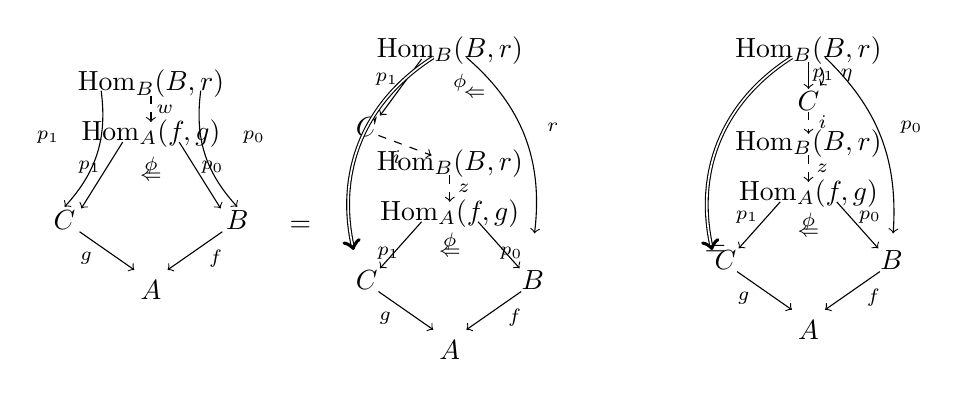
\begin{tikzpicture}[x=1.2em,y=1.2em]
  \node (hb) at (0,4.0) {$\mathrm{Hom}_B(B,r)$};
  \draw[->,dashed] (0,3.65) -- (0,2.85);
  \node at (0.42,3.25) {$\scriptstyle w$};
  \node (ha) at (0,2.5) {$\mathrm{Hom}_A(f,g)$};
  \draw[->] (-1.5,3.8) to[bend left=25] (-2.6,0.3);
  \node at (-3.1,2.4) {$\scriptstyle p_{1}$};
  \draw[->] (1.5,3.8) to[bend right=25] (2.6,0.3);
  \node at (3.1,2.4) {$\scriptstyle p_{0}$};
  \node (c) at (-2.6,-0.1) {$C$};
  \node (b) at (2.6,-0.1) {$B$};
  \draw[->] (-0.85,2.25) -- (-2.1,0.25);
  \node at (-1.85,1.5) {$\scriptstyle p_{1}$};
  \draw[->] (0.85,2.25) -- (2.1,0.25);
  \node at (1.85,1.5) {$\scriptstyle p_{0}$};
  \node at (0,1.55) {$\scriptstyle\phi$};
  \node at (0,1.21) {$\scriptstyle\Leftarrow$};
  \draw[->] (-2.15,-0.45) -- (-0.5,-1.6);
  \node at (-1.95,-1.25) {$\scriptstyle g$};
  \draw[->] (2.15,-0.45) -- (0.5,-1.6);
  \node at (1.95,-1.25) {$\scriptstyle f$};
  \node (a) at (0,-2.2) {$A$};
  \node at (4.5,-0.3) {$=$};
  \begin{scope}[shift={(9.0,0)}]
  \node (hb) at (0,5.0) {$\mathrm{Hom}_B(B,r)$};
  \draw[->] (-0.85,4.75) -- (-2.1,3.05);
  \node at (-1.9,4.15) {$\scriptstyle p_{1}$};
  \node at (0.3,4.05) {$\scriptstyle\phi$};
  \node at (0.75,3.71) {$\scriptstyle\Leftarrow$};
  \node (cm) at (-2.5,2.7) {$C$};
  \draw[double,->] (-0.5,4.8) to[bend right=35] (-2.9,-1.0);
  \draw[->] (0.5,4.8) to[bend left=28] (2.55,-0.5);
  \node at (3.1,2.7) {$\scriptstyle r$};
  \draw[->,dashed] (-2.15,2.45) -- (-0.55,1.85);
  \node at (-1.6,1.8) {$\scriptstyle i$};
  \node (h2) at (0,1.6) {$\mathrm{Hom}_B(B,r)$};
  \draw[->,dashed] (0,1.25) -- (0,0.45);
  \node at (0.42,0.85) {$\scriptstyle z$};
  \node (ha) at (0,0.1) {$\mathrm{Hom}_A(f,g)$};
  \node (c) at (-2.5,-1.9) {$C$};
  \node (b) at (2.5,-1.9) {$B$};
  \draw[->] (-0.85,-0.15) -- (-2.1,-1.55);
  \node at (-1.85,-1.1) {$\scriptstyle p_{1}$};
  \draw[->] (0.85,-0.15) -- (2.1,-1.55);
  \node at (1.85,-1.1) {$\scriptstyle p_{0}$};
  \node at (0,-0.75) {$\scriptstyle\phi$};
  \node at (0,-1.09) {$\scriptstyle\Leftarrow$};
  \draw[->] (-2.15,-2.25) -- (-0.5,-3.4);
  \node at (-1.95,-3.05) {$\scriptstyle g$};
  \draw[->] (2.15,-2.25) -- (0.5,-3.4);
  \node at (1.95,-3.05) {$\scriptstyle f$};
  \node (a) at (0,-4.0) {$A$};
  \end{scope}
  \node at (17.0,-1.0) {$=$};
  \begin{scope}[shift={(19.8,0)}]
  \node (hb) at (0,5.0) {$\mathrm{Hom}_B(B,r)$};
  \draw[->] (0,4.65) -- (0,3.85);
  \node at (0.45,4.25) {$\scriptstyle p_{1}$};
  \draw[->] (0.35,4.5) to[bend left=40] (0.35,3.95);
  \node at (1.15,4.25) {$\scriptstyle\eta$};
  \node (cm) at (0,3.5) {$C$};
  \draw[double,->] (-0.5,4.8) to[bend right=35] (-2.9,-1.0);
  \draw[->] (0.5,4.8) to[bend left=25] (2.55,-0.5);
  \node at (3.1,2.7) {$\scriptstyle p_{0}$};
  \draw[->,dashed] (0,3.15) -- (0,2.5);
  \node at (0.42,2.85) {$\scriptstyle i$};
  \node (h2) at (0,2.2) {$\mathrm{Hom}_B(B,r)$};
  \draw[->,dashed] (0,1.85) -- (0,1.05);
  \node at (0.42,1.45) {$\scriptstyle z$};
  \node (ha) at (0,0.7) {$\mathrm{Hom}_A(f,g)$};
  \node (c) at (-2.5,-1.3) {$C$};
  \node (b) at (2.5,-1.3) {$B$};
  \draw[->] (-0.85,0.45) -- (-2.1,-0.95);
  \node at (-1.85,0.0) {$\scriptstyle p_{1}$};
  \draw[->] (0.85,0.45) -- (2.1,-0.95);
  \node at (1.85,0.0) {$\scriptstyle p_{0}$};
  \node at (0,-0.15) {$\scriptstyle\phi$};
  \node at (0,-0.49) {$\scriptstyle\Leftarrow$};
  \draw[->] (-2.15,-1.65) -- (-0.5,-2.8);
  \node at (-1.95,-2.45) {$\scriptstyle g$};
  \draw[->] (2.15,-1.65) -- (0.5,-2.8);
  \node at (1.95,-2.45) {$\scriptstyle f$};
  \node (a) at (0,-3.4) {$A$};
  \end{scope}
\end{tikzpicture}
\end{center}
由\cref{lem:right-adjoint-right-inverse}，存在\trNaturalTransformation{} $\eta\colon\mathrm{id}\Rightarrow ip_{1}$ %
使得 $p_{0}\eta=\phi$——这给出上中的粘贴等式——且 $p_{1}\eta=\mathrm{id}$，后者告诉我们%
右侧粘贴图约化为 $\phi z$。命题 3.4.7 现在蕴含：在 $C\times B$ 上 $w\cong z$。
\end{proof}

\cref{thm:trio-bijection}的一个对偶版本把\trNaturalTransformation{} $g\Rightarrow g\ell$ 表示为居于%
$B\times C$ 之上的映射 $\mathrm{Hom}_B(\ell,B)\to\mathrm{Hom}_A(g,f)$ 的%
\trFiberedIsomorphism{}类。把这些结果特殊化到 $f$ 或 $g$ 之一为恒同的情形，%
我们立即复原出「廉价」形式的\trYonedaLemma{}：

\begin{corollary}\label{cor:cheap-yoneda}
给定一平行\trFunctor{}对 $f,g\colon A\to B$，在下中所示的\trNaturalTransformation{}与它们的左表示、%
右表示作为\trCommaInfinityCategory{}之间的映射的\trFiberedIsomorphism{}类——如下左与下右所示——%
之间，存在双射
\begin{center}
\begin{tikzpicture}[x=1.4em,y=1.4em]
  \node at (0,0) {%
  $\left\{\vcenter{\hbox{\begin{tikzpicture}[x=1.3em,y=1.3em]
    \node (hg) at (0,2.6) {$\mathrm{Hom}_B(g,B)$};
    \node (b) at (-2.4,0.8) {$B$};
    \node (a) at (2.4,0.8) {$A$};
    \draw[->] (-0.85,2.35) -- (-1.95,1.15);
    \node at (-1.85,2.0) {$\scriptstyle p_{1}$};
    \draw[->] (0.85,2.35) -- (1.95,1.15);
    \node at (1.85,2.0) {$\scriptstyle p_{0}$};
    \draw[->,dashed] (0,2.25) -- (0,-0.15);
    \node at (0.95,1.05) {$\scriptstyle\qcor{\alpha^{*}}$};
    \node (hf) at (0,-0.5) {$\mathrm{Hom}_B(f,B)$};
    \draw[->] (-0.85,-0.75) -- (-1.95,0.45);
    \node at (-1.85,-1.0) {$\scriptstyle p_{1}$};
    \draw[->] (0.85,-0.75) -- (1.95,0.45);
    \node at (1.85,-1.0) {$\scriptstyle p_{0}$};
  \end{tikzpicture}}}\right\}_{/\cong}$};
  \node at (4.8,0.6) {$\longleftrightarrow$};
  \node at (8.4,0.6) {%
  $\left\{\vcenter{\hbox{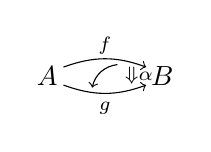
\begin{tikzpicture}[x=1.3em,y=1.3em]
    \node (a) at (-1.6,0) {$A$};
    \node (b) at (1.6,0) {$B$};
    \draw[->] (-1.15,0.25) to[bend left=20] (1.15,0.25);
    \node at (0,0.85) {$\scriptstyle f$};
    \draw[->] (-1.15,-0.25) to[bend right=20] (1.15,-0.25);
    \node at (0,-0.9) {$\scriptstyle g$};
    \draw[->] (0.35,0.32) to[bend right=35] (-0.35,-0.32);
    \node at (0.95,0.0) {$\scriptstyle\Downarrow\alpha$};
  \end{tikzpicture}}}\right\}$};
  \node at (12.0,0.6) {$\longleftrightarrow$};
  \node at (15.8,0.6) {%
  $\left\{\vcenter{\hbox{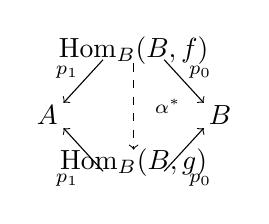
\begin{tikzpicture}[x=1.3em,y=1.3em]
    \node (hb) at (0,2.6) {$\mathrm{Hom}_B(B,f)$};
    \node (a) at (-2.4,0.8) {$A$};
    \node (b) at (2.4,0.8) {$B$};
    \draw[->] (-0.85,2.35) -- (-1.95,1.15);
    \node at (-1.85,2.0) {$\scriptstyle p_{1}$};
    \draw[->] (0.85,2.35) -- (1.95,1.15);
    \node at (1.85,2.0) {$\scriptstyle p_{0}$};
    \draw[->,dashed] (0,2.25) -- (0,-0.15);
    \node at (0.95,1.05) {$\scriptstyle\qcor{\alpha^{*}}$};
    \node (hg) at (0,-0.5) {$\mathrm{Hom}_B(B,g)$};
    \draw[->] (-0.85,-0.75) -- (-1.95,0.45);
    \node at (-1.85,-1.0) {$\scriptstyle p_{1}$};
    \draw[->] (0.85,-0.75) -- (1.95,0.45);
    \node at (1.85,-1.0) {$\scriptstyle p_{0}$};
  \end{tikzpicture}}}\right\}_{/\cong}$};
\end{tikzpicture}
\end{center}
这些双射分别由与 $g$ 之上的左\trCommaCone{}和 $f$ 之上的右\trCommaCone{}作粘贴
\begin{center}
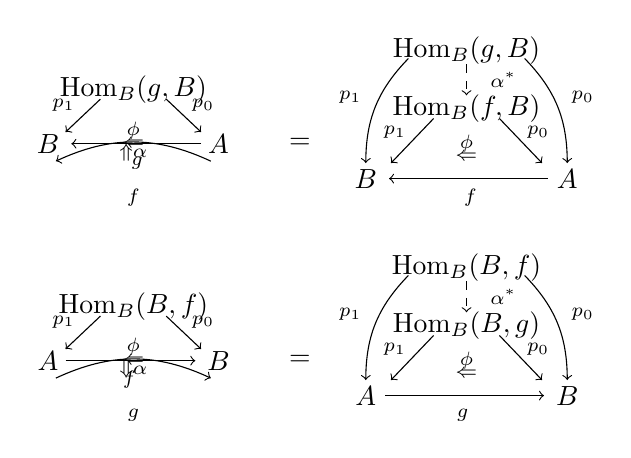
\begin{tikzpicture}[x=1.4em,y=1.4em]
  \node (hom) at (0,2.4) {$\mathrm{Hom}_B(g,B)$};
  \node (b) at (-2.2,1.0) {$B$};
  \node (a) at (2.2,1.0) {$A$};
  \draw[->] (-0.85,2.15) -- (-1.75,1.3);
  \node at (-1.8,2.0) {$\scriptstyle p_{1}$};
  \draw[->] (0.85,2.15) -- (1.75,1.3);
  \node at (1.8,2.0) {$\scriptstyle p_{0}$};
  \node at (0,1.35) {$\scriptstyle\phi$};
  \node at (0,1.01) {$\scriptstyle\Leftarrow$};
  \draw[->] (1.75,1.0) -- (-1.6,1.0);
  \node at (0.1,0.5) {$\scriptstyle g$};
  \draw[->] (2.0,0.55) to[bend right=25] (-2.0,0.55);
  \node at (0,-0.4) {$\scriptstyle f$};
  \node at (0,0.76) {$\scriptstyle\Uparrow\alpha$};
  \node at (4.3,1.0) {$=$};
  \begin{scope}[shift={(8.6,0)}]
  \node (hg) at (0,3.4) {$\mathrm{Hom}_B(g,B)$};
  \draw[->,dashed] (0,3.05) -- (0,2.25);
  \node at (0.95,2.65) {$\scriptstyle\qcor{\alpha^{*}}$};
  \node (hf) at (0,1.9) {$\mathrm{Hom}_B(f,B)$};
  \draw[->] (-1.5,3.2) to[bend right=22] (-2.6,0.5);
  \node at (-3.0,2.2) {$\scriptstyle p_{1}$};
  \draw[->] (1.5,3.2) to[bend left=22] (2.6,0.5);
  \node at (3.0,2.2) {$\scriptstyle p_{0}$};
  \node (b) at (-2.6,0.1) {$B$};
  \node (a) at (2.6,0.1) {$A$};
  \draw[->] (-0.85,1.65) -- (-1.95,0.5);
  \node at (-1.85,1.3) {$\scriptstyle p_{1}$};
  \draw[->] (0.85,1.65) -- (1.95,0.5);
  \node at (1.85,1.3) {$\scriptstyle p_{0}$};
  \node at (0,1.0) {$\scriptstyle\phi$};
  \node at (0,0.66) {$\scriptstyle\Leftarrow$};
  \draw[->] (2.1,0.1) -- (-2.0,0.1);
  \node at (0.1,-0.4) {$\scriptstyle f$};
  \end{scope}
  \begin{scope}[shift={(0,-5.6)}]
  \node (hom) at (0,2.4) {$\mathrm{Hom}_B(B,f)$};
  \node (a) at (-2.2,1.0) {$A$};
  \node (b) at (2.2,1.0) {$B$};
  \draw[->] (-0.85,2.15) -- (-1.75,1.3);
  \node at (-1.8,2.0) {$\scriptstyle p_{1}$};
  \draw[->] (0.85,2.15) -- (1.75,1.3);
  \node at (1.8,2.0) {$\scriptstyle p_{0}$};
  \node at (0,1.35) {$\scriptstyle\phi$};
  \node at (0,1.01) {$\scriptstyle\Leftarrow$};
  \draw[->] (-1.75,1.0) -- (1.6,1.0);
  \node at (-0.1,0.5) {$\scriptstyle f$};
  \draw[->] (-2.0,0.55) to[bend left=25] (2.0,0.55);
  \node at (0,-0.4) {$\scriptstyle g$};
  \node at (0,0.76) {$\scriptstyle\Downarrow\alpha$};
  \node at (4.3,1.0) {$=$};
  \begin{scope}[shift={(8.6,0)}]
  \node (hb) at (0,3.4) {$\mathrm{Hom}_B(B,f)$};
  \draw[->,dashed] (0,3.05) -- (0,2.25);
  \node at (0.95,2.65) {$\scriptstyle\qcor{\alpha^{*}}$};
  \node (hg) at (0,1.9) {$\mathrm{Hom}_B(B,g)$};
  \draw[->] (-1.5,3.2) to[bend right=22] (-2.6,0.5);
  \node at (-3.0,2.2) {$\scriptstyle p_{1}$};
  \draw[->] (1.5,3.2) to[bend left=22] (2.6,0.5);
  \node at (3.0,2.2) {$\scriptstyle p_{0}$};
  \node (a) at (-2.6,0.1) {$A$};
  \node (b) at (2.6,0.1) {$B$};
  \draw[->] (-0.85,1.65) -- (-1.95,0.5);
  \node at (-1.85,1.3) {$\scriptstyle p_{1}$};
  \draw[->] (0.85,1.65) -- (1.95,0.5);
  \node at (1.85,1.3) {$\scriptstyle p_{0}$};
  \node at (0,1.0) {$\scriptstyle\phi$};
  \node at (0,0.66) {$\scriptstyle\Leftarrow$};
  \draw[->] (-2.1,0.1) -- (2.0,0.1);
  \node at (-0.1,-0.4) {$\scriptstyle g$};
  \end{scope}
  \end{scope}
\end{tikzpicture}
\end{center}
再应用\trOneCellInduction{}穿过前一种情形的左\trCommaCone{}或后一种情形的右\trCommaCone{}作因子分解%
而构造。
\end{corollary}

组合本节的诸结果，我们证明最后一个可表示性定理，使我们能够在没有预定表示\trFunctor{}的%
情形下识别一个\trCommaInfinityCategory{}何时右可表示。这一结果特殊化后给出下一章中伴随\trFunctor{}的%
存在定理以及\trLimit{}与\trColimit{}的存在定理。

\begin{theorem}\label{thm:right-representability}
与\trCospan{} $C\xrightarrow{\;g\;}A\xleftarrow{\;f\;}B$ 相伴的\trCommaInfinityCategory{} $\mathrm{Hom}_A(f,g)$ %
是右可表示的，当且仅当其余定义域投影函子具有一个\trRightAdjoint\trRightInverse{}
\begin{center}
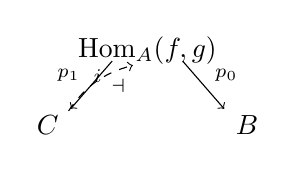
\begin{tikzpicture}[x=1.5em,y=1.5em]
  \node (hom) at (0,2.2) {$\mathrm{Hom}_A(f,g)$};
  \node (c) at (-2.4,0.4) {$C$};
  \node (b) at (2.4,0.4) {$B$};
  \draw[->] (-0.85,1.95) -- (-1.85,0.8);
  \node at (-1.9,1.6) {$\scriptstyle p_{1}$};
  \node at (-0.7,1.35) {$\scriptstyle\dashv$};
  \draw[->] (0.85,1.95) -- (1.85,0.8);
  \node at (1.9,1.6) {$\scriptstyle p_{0}$};
  \draw[->,dashed] (-1.9,0.75) to[bend left=20] (-0.35,1.85);
  \node at (-1.2,1.6) {$\scriptstyle i$};
\end{tikzpicture}
\end{center}
此时复合 $p_{0}i\colon C\to B$ 定义表示\trFunctor{}，而由\trFunctor{} %
$i\colon C\to\mathrm{Hom}_A(f,g)$ 所编码的\trNaturalTransformation{}定义 $g$ 穿过 $f$ 的一个绝对右提升。
\end{theorem}

\begin{proof}
设\trCommaInfinityCategory{} $\mathrm{Hom}_A(f,g)$ 由\trFunctor{} $r\colon C\to B$ 右表示。由%
\cref{lem:right-adjoint-right-inverse}，$p_{1}\colon\mathrm{Hom}_B(B,r)\twoheadrightarrow C$ %
具有\trRightAdjoint\trRightInverse{} $i'$，它与\trFiberedEquivalence{}复合，便为与之\trEquivalence{}的%
\trFunctor{} $p_{1}\colon\mathrm{Hom}_A(f,g)\twoheadrightarrow C$ 定义一个\trRightAdjoint\trRightInverse{}
\begin{center}
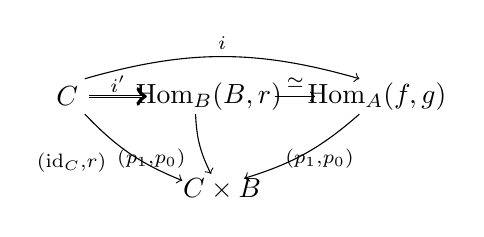
\begin{tikzpicture}[x=1.6em,y=1.6em]
  \node (c) at (-3.4,0.9) {$C$};
  \node (h1) at (-0.2,0.9) {$\mathrm{Hom}_B(B,r)$};
  \node (h2) at (3.6,0.9) {$\mathrm{Hom}_A(f,g)$};
  \draw[->] (-3.0,1.3) to[bend left=16] (3.2,1.3);
  \node at (0.1,2.1) {$\scriptstyle i$};
  \draw[double,->] (-2.9,0.9) -- (-1.6,0.9);
  \node at (-2.25,1.18) {$\scriptstyle i'$};
  \draw[->] (1.3,0.9) -- (2.2,0.9);
  \node at (1.75,1.2) {$\scriptstyle\simeq$};
  \node (cb) at (0.1,-1.2) {$C\times B$};
  \draw[->] (-0.5,0.5) to[bend right=12] (-0.15,-0.85);
  \node at (-1.5,-0.5) {$\scriptstyle(p_{1},p_{0})$};
  \draw[->] (3.2,0.5) to[bend left=12] (0.6,-0.95);
  \node at (2.3,-0.5) {$\scriptstyle(p_{1},p_{0})$};
  \draw[->] (-3.0,0.5) to[bend right=12] (-0.8,-1.0);
  \node at (-3.3,-0.6) {$\scriptstyle(\mathrm{id}_C,r)$};
\end{tikzpicture}
\end{center}
注意 $r=p_{0}i$，且据\cref{thm:trio-bijection}之证明中的构造，\trFunctor{} %
$i\colon C\to\mathrm{Hom}_A(f,g)$ 编码一个绝对右提升图表 $\rho\colon fr\Rightarrow g$。%
\footnote{原书印作「$\rho\colon rf\Rightarrow g$」，疑为「$fr$」之误，此处径改。%
——译者注}于是只剩逆方向待证。

为此，设给定一个\trRightAdjoint\trRightInverse{}\trAdjunction{} $p_{1}\dashv i$。展开定义，这供给 $C$ 之上的一个\trAdjunction{}
\begin{center}
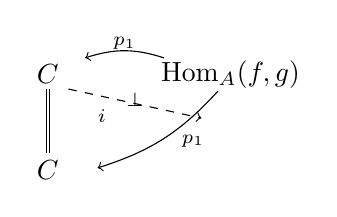
\begin{tikzpicture}[x=1.5em,y=1.5em]
  \node (c1) at (-1.8,1.4) {$C$};
  \node (h) at (2.6,1.4) {$\mathrm{Hom}_A(f,g)$};
  \draw[->] (1.0,1.8) to[bend right=18] (-0.9,1.8);
  \node at (0.05,2.16) {$\scriptstyle p_{1}$};
  \node at (0.3,0.8) {$\scriptstyle\perp$};
  \draw[->,dashed] (-1.3,1.05) -- (1.9,0.35);
  \node at (-0.5,0.4) {$\scriptstyle i$};
  \draw[double] (-1.8,1.05) -- (-1.8,-0.5);
  \node (c2) at (-1.8,-0.9) {$C$};
  \draw[->] (2.3,1.0) to[bend left=15] (-0.6,-0.85);
  \node at (1.7,-0.2) {$\scriptstyle p_{1}$};
\end{tikzpicture}
\end{center}
其\trCounit{}是恒同，其\trUnit{} $\eta\colon\mathrm{id}\Rightarrow ip_{1}$ 满足条件 %
$\eta i=\mathrm{id}_i$ 与 $p_{1}\eta=\mathrm{id}_{p_{1}}$。由\cref{thm:trio-bijection}，%
为构造\trFiberedEquivalence{} $\mathrm{Hom}_B(B,r)\simeq_{C\times B}\mathrm{Hom}_A(f,g)$——取 %
$r:=p_{0}i$——只需证明：把 $\mathrm{Hom}_A(f,g)$ 的\trCommaCone{}沿 $i$ 限制所得的\trNaturalTransformation{}
\begin{center}
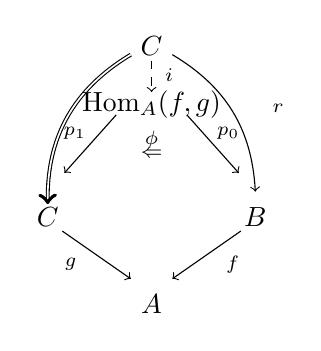
\begin{tikzpicture}[x=1.5em,y=1.5em]
  \node (ctop) at (0,3.4) {$C$};
  \draw[double,->] (-0.5,3.2) to[bend right=30] (-2.5,-0.4);
  \draw[->,dashed] (0,3.05) -- (0,2.3);
  \node at (0.42,2.7) {$\scriptstyle i$};
  \node (ha) at (0,2.0) {$\mathrm{Hom}_A(f,g)$};
  \draw[->] (0.5,3.2) to[bend left=28] (2.5,-0.1);
  \node at (3.05,1.9) {$\scriptstyle r$};
  \node (c) at (-2.5,-0.7) {$C$};
  \node (b) at (2.5,-0.7) {$B$};
  \draw[->] (-0.85,1.75) -- (-2.1,0.35);
  \node at (-1.85,1.3) {$\scriptstyle p_{1}$};
  \draw[->] (0.85,1.75) -- (2.1,0.35);
  \node at (1.85,1.3) {$\scriptstyle p_{0}$};
  \node at (0,1.15) {$\scriptstyle\phi$};
  \node at (0,0.81) {$\scriptstyle\Leftarrow$};
  \draw[->] (-2.15,-1.05) -- (-0.5,-2.2);
  \node at (-1.95,-1.85) {$\scriptstyle g$};
  \draw[->] (2.15,-1.05) -- (0.5,-2.2);
  \node at (1.95,-1.85) {$\scriptstyle f$};
  \node (a) at (0,-2.8) {$A$};
\end{tikzpicture}
\end{center}
定义一个绝对右提升图表。

由\trOneCellInduction{}，任何\trNaturalTransformation{} $\chi\colon fb\Rightarrow gc$ 诱导一个\trFunctor{}%
$\qcor{\chi}$，如下左所示：
\begin{center}
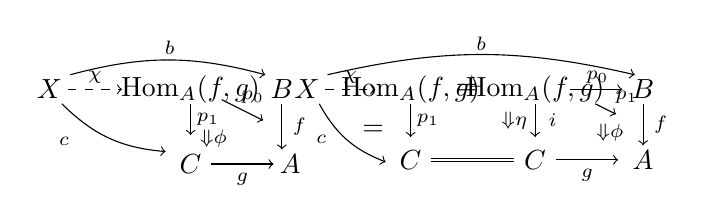
\begin{tikzpicture}[x=1.5em,y=1.5em]
  \node (x) at (-3.2,1.6) {$X$};
  \draw[->,dashed] (-2.75,1.6) -- (-1.45,1.6);
  \node at (-2.1,1.9) {$\scriptstyle\qcor{\chi}$};
  \node (hom) at (0.2,1.6) {$\mathrm{Hom}_A(f,g)$};
  \draw[->] (-2.7,1.95) to[bend left=15] (2.0,1.95);
  \node at (-0.3,2.6) {$\scriptstyle b$};
  \node (b) at (2.4,1.6) {$B$};
  \draw[->] (0.95,1.35) -- (1.95,0.85);
  \node at (1.7,1.4) {$\scriptstyle p_{0}$};
  \draw[->] (0.2,1.25) -- (0.2,0.5);
  \node at (0.62,0.88) {$\scriptstyle p_{1}$};
  \node at (0.75,0.4) {$\scriptstyle\Downarrow\phi$};
  \draw[->] (-2.9,1.25) to[bend right=20] (-0.4,0.1);
  \node at (-2.85,0.35) {$\scriptstyle c$};
  \node (c) at (0.2,-0.2) {$C$};
  \draw[->] (0.7,-0.2) -- (2.2,-0.2);
  \node at (1.45,-0.56) {$\scriptstyle g$};
  \node (a) at (2.6,-0.2) {$A$};
  \draw[->] (2.4,1.25) -- (2.4,0.15);
  \node at (2.82,0.7) {$\scriptstyle f$};
  \node at (4.6,0.6) {$=$};
  \begin{scope}[shift={(7.4,0)}]
  \node (x) at (-4.4,1.6) {$X$};
  \draw[->,dashed] (-3.95,1.6) -- (-2.75,1.6);
  \node at (-3.35,1.9) {$\scriptstyle\qcor{\chi}$};
  \node (h1) at (-1.9,1.6) {$\mathrm{Hom}_A(f,g)$};
  \node (eq) at (-0.55,1.6) {$=$};
  \node (h2) at (1.1,1.6) {$\mathrm{Hom}_A(f,g)$};
  \node (b) at (3.7,1.6) {$B$};
  \draw[->] (1.95,1.6) -- (3.2,1.6);
  \node at (2.6,1.88) {$\scriptstyle p_{0}$};
  \draw[->] (-3.9,1.95) to[bend left=13] (3.5,1.95);
  \node at (-0.2,2.7) {$\scriptstyle b$};
  \draw[->] (-1.9,1.25) -- (-1.9,0.45);
  \node at (-1.48,0.85) {$\scriptstyle p_{1}$};
  \draw[->] (1.1,1.25) -- (1.1,0.45);
  \node at (0.6,0.85) {$\scriptstyle\Downarrow\eta$};
  \node at (1.52,0.85) {$\scriptstyle i$};
  \draw[->] (2.55,1.25) -- (3.05,1.0);
  \node at (3.3,1.4) {$\scriptstyle p_{1}$};
  \node at (2.9,0.55) {$\scriptstyle\Downarrow\phi$};
  \node (c1) at (-1.9,-0.1) {$C$};
  \node (c2) at (1.1,-0.1) {$C$};
  \draw[double] (-1.4,-0.1) -- (0.6,-0.1);
  \draw[->] (1.6,-0.1) -- (3.1,-0.1);
  \node at (2.35,-0.46) {$\scriptstyle g$};
  \node (a) at (3.7,-0.1) {$A$};
  \draw[->] (3.7,1.25) -- (3.7,0.25);
  \node at (4.12,0.75) {$\scriptstyle f$};
  \draw[->] (-4.1,1.25) to[bend right=20] (-2.5,-0.15);
  \node at (-4.05,0.4) {$\scriptstyle c$};
  \end{scope}
\end{tikzpicture}
\end{center}
把\trTriangleEqualities{} $p_{1}\eta=\mathrm{id}_{p_{1}}$ 按上右所示插入，便构造出所要的因子分解——%
$\chi$ 穿过 $\phi i$ 的因子分解 $p_{0}\eta\qcor{\chi}\colon b\Rightarrow rc$。

事实上，给定任何定义了 $\chi\colon fb\Rightarrow gc$ 穿过 $\phi i$ 的因子分解的%
\trNaturalTransformation{} $\tau_{0}\colon b\Rightarrow rc$，二元组 $(\mathrm{id}_c,\tau_{0})$ 满足%
命题 3.4.6(ii) 的相容性条件，从而诱导\trNaturalTransformation{} $\tau\colon\qcor{\chi}\Rightarrow ic$，%
使得 $\mathrm{id}_c=p_{1}\tau$ 且 $\tau_{0}=p_{0}\tau$。我们论证\trNaturalTransformation{} $\tau$ 唯一，%
从而证明因子分解 $p_{0}\tau\colon b\Rightarrow rc$ 也唯一。

为见此，注意 $C$ 之上的\trAdjunction{} $p_{1}\dashv i$ 把\trRightAdjoint{}展示为对象 %
$p_{1}\colon\mathrm{Hom}_A(f,g)\to C$ 在\trHomotopyTwoCategory{}的 $C$ 上的%
\textbf{严格切片}（strict slice）中的一个\trTerminal{}元素。\footnote{对象是∞-范畴%
的\trFunctor{} $c\colon X\to C$；1-\trCell{}是定义域∞-范畴之间的、定义一个严格交换%
三角形的\trFunctor{}；2-\trCell{}是这些\trFunctor{}之间的\trNaturalTransformation{}，其\trWhiskering{}后%
定义一个余定义域为 $C$ 的恒同 2-\trCell{}。}据第 2 章中的引理 2.2.5 之理，对任何对象%
$c\colon X\to C$ 与任何居于 $C$ 之上的态射 $\qcor{\chi}\colon X\to\mathrm{Hom}_A(f,g)$，%
存在唯一的、居于 $C$ 之上的\trNaturalTransformation{} $\qcor{\chi}\Rightarrow ic$。于是，存在唯一的\trNaturalTransformation{} %
$\tau\colon\qcor{\chi}\Rightarrow ic$ 具有性质 $p_{1}\tau=\mathrm{id}_c$，从而 %
$\chi$ 穿过 $\phi i$ 的因子分解 $p_{0}\tau\colon b\Rightarrow rc$ 也必唯一。
\end{proof}

在下一节中，我们将发现：\cref{thm:right-representability}可以更简洁地表述为如下断言：%
∞-宇宙 $\mathcal{K}$ 中的\trCommaInfinityCategory{} $\mathrm{Hom}_A(f,g)$ 是右可表示的，恰好当其余%
定义域投影函子 $p_{1}\colon\mathrm{Hom}_A(f,g)\twoheadrightarrow C$ 作为\trSliceInfinityCosmos{}%
$\mathcal{K}_{/C}$ 的一个对象具有一个\trTerminal{}元素时（见推论 3.6.10）。对偶地，%
$\mathrm{Hom}_A(f,g)$ 是左可表示的，恰好当其定义域投影函子作为\trSliceInfinityCosmos{} %
$\mathcal{K}_{/B}$ 的一个对象具有一个\trInitial{}元素时。
这一陈述与\cref{thm:right-representability}所证的版本之间有一道小缝隙，涉及\trSliceInfinityCosmos{}%
$\mathcal{K}_{/C}$ 的\trHomotopyTwoCategory{}与\trHomotopyTwoCategory{} %
$\mathbb{h}\mathcal{K}$ 在 $C$ 上的切片之间的分歧。这正是我们接下来要讨论的主题。

\subsection*{练习}

\begin{exercise}\label{ex:anticipate-adjunction}
通过探索如何用\trCommaInfinityCategory{}编码一个给定的对立\trFunctor{}对之间的\trAdjunction{} $f\dashv u$ 的存在性，%
以预期第 4 章中的命题 4.1.1。
\end{exercise}

\begin{exercise}\label{ex:cospans-equivalence-absrl}
把练习 2.3.vi 的结果扩充以证明：对\trCospan{}的任何\trEquivalence
\begin{center}
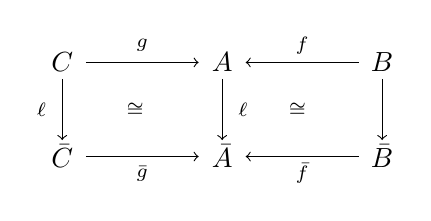
\begin{tikzpicture}[x=1.7em,y=1.7em]
  \node (c) at (0,1.3) {$C$};
  \node (a) at (3.4,1.3) {$A$};
  \node (b) at (6.8,1.3) {$B$};
  \node (cb) at (0,-0.7) {$\bar{C}$};
  \node (ab) at (3.4,-0.7) {$\bar{A}$};
  \node (bb) at (6.8,-0.7) {$\bar{B}$};
  \draw[->] (0.5,1.3) -- (2.9,1.3);
  \node at (1.7,1.66) {$\scriptstyle g$};
  \draw[->] (6.3,1.3) -- (3.9,1.3);
  \node at (5.1,1.66) {$\scriptstyle f$};
  \draw[->] (0.5,-0.7) -- (2.9,-0.7);
  \node at (1.7,-1.06) {$\scriptstyle\bar{g}$};
  \draw[->] (6.3,-0.7) -- (3.9,-0.7);
  \node at (5.1,-1.06) {$\scriptstyle\bar{f}$};
  \draw[->] (0,0.95) -- (0,-0.35);
  \node at (-0.44,0.3) {$\scriptstyle\ell$};
  \draw[->] (3.4,0.95) -- (3.4,-0.35);
  \node at (3.84,0.3) {$\scriptstyle\ell$};
  \draw[->] (6.8,0.95) -- (6.8,-0.35);
  \node at (1.55,0.3) {$\scriptstyle\cong$};
  \node at (5.0,0.3) {$\scriptstyle\cong$};
\end{tikzpicture}
\end{center}
$g$ 穿过 $f$ 的绝对右提升存在，当且仅当 $\bar{g}$ 穿过 $\bar{f}$ 的绝对右提升存在。
\end{exercise}

\begin{exercise}\label{ex:fully-faithful-reflects-limits}
（文献 [124, 3.7]）利用\cref{thm:absrl-equivalence}与\cref{cor:fully-faithful}(iv) 证明：一个\trFullyFaithful%
\trFunctor{} $f\colon A\to B$ 反射 $A$ 中存在的所有\trLimit{}或\trColimit{}。为什么%
这一论证不能同样证明 $f\colon A\to B$ 保持它们？
\end{exercise}
